\documentclass[11pt]{article}
\usepackage[T1]{fontenc}
\usepackage{lmodern}
\usepackage[margin=1in]{geometry}
\usepackage{amsmath,amssymb,amsthm,mathtools}
\usepackage{booktabs,array,enumitem,graphicx}
\usepackage[numbers,sort&compress]{natbib}
\usepackage[colorlinks=true,allcolors=blue]{hyperref}
\usepackage[nameinlink,noabbrev]{cleveref}
\newtheorem{theorem}{Theorem}[section]
\newtheorem{proposition}[theorem]{Proposition}
\newtheorem{lemma}[theorem]{Lemma}
\newtheorem{corollary}[theorem]{Corollary}
\theoremstyle{definition}
\newtheorem{definition}[theorem]{Definition}
\newtheorem{example}[theorem]{Example}
\theoremstyle{remark}
\newtheorem{remark}[theorem]{Remark}
\newcommand{\R}{\mathbb R}
\newcommand{\C}{\mathbb C}
\newcommand{\F}{\mathbb F}
\newcommand{\N}{\mathbb N}
\newcommand{\ip}[2]{\langle #1,#2\rangle}
\newcommand{\norm}[1]{\lVert #1\rVert}
\newcommand{\abs}[1]{\lvert #1\rvert}
\newcommand{\dd}{\,\mathrm d}
\newcommand{\SC}{\mathrm{sc}}
\newcommand{\CP}{\mathrm{CP}}
\newcommand{\opt}{\mathrm{opt}}
\newcommand{\op}{\mathrm{op}}
\newcommand{\diag}{\operatorname{diag}}
\newcommand{\tr}{\operatorname{tr}}
\newcommand{\rank}{\operatorname{rank}}
\newcommand{\sgn}{\operatorname{sgn}}
\newcommand{\Len}{\operatorname{len}}
\newcommand{\interior}{\operatorname{int}}
\newcommand{\argmin}{\operatorname*{arg\,min}}
\newcommand{\pos}[1]{[#1]_+}
\newcommand{\ball}{\mathcal B}
\newcommand{\gap}{\operatorname{gap}}
\newcommand{\eps}{\varepsilon}
\numberwithin{equation}{section}
\allowdisplaybreaks[2]

\title{The Cost of Following the Central Path}
\author{}
\date{}
\hypersetup{
 pdftitle={The Cost of Following the Central Path},
 pdfsubject={Central-path movement in self-concordant barrier Hessian metrics},
 pdfkeywords={interior-point methods; self-concordant barriers; central path; Riemannian distance; spectral optimization}
}
\begin{document}
\maketitle
\begin{abstract}
Interior-point methods take bounded steps in the local Hessian norm of
a self-concordant barrier; up to constants, the least number of such
steps between two points is their distance in the Hessian metric.
We ask how much longer the central path is, in this metric, than the
shortest route from the analytic center to a point whose objective value
is within $\eps$ of the optimum. For boxes, spectral-norm balls of real
and complex matrices, spectral intervals of Euclidean Jordan
algebras, and products of these domains, with their standard logarithmic and log-determinant barriers,
we compute these distances exactly. If all factors have the same
barrier coefficient and the linear objective has $r$ nonzero singular
values or eigenvalues (coefficients, for a box), every arc of the central
path has length at most
$\Gamma_r=[\sum_{i=1}^r(\sqrt i-\sqrt{i-1})^2]^{1/2}$
times the distance between its endpoints, where
$\Gamma_r^2=\frac14\log r+O(1)$, and no smaller constant works. The
central path to its first $\eps$-accurate point has length at most
$c_\star\Gamma_r$ times the distance to the set of $\eps$-accurate
points, where $1.37486<c_\star<1.38$.
For an explicit sparse linear program on $(-1,1)^r$ with
rational data and tolerance $\eps_r=e^{-\Theta(r)}$, the least number of bounded steps
from the analytic center to an $\eps_r$-accurate point is
$\Theta(r\sqrt{\log r})$, but $\Theta(r\log r)$ if every iterate must
stay within a fixed Hessian-metric distance of the central path. The
same gap, a factor $\Theta(\sqrt{\log r})$, holds for the universal and
entropic barriers of the cube and, uniformly in its parameters, for a
family of non-separable barriers on the cube with the least possible
barrier parameter $r$. On the same program, reaching a strictly feasible
primal--dual pair with small duality gap takes $\Theta(r^{3/2})$ steps
in the primal--dual barrier metric. We count bounded steps, not
arithmetic or oracle cost.
\end{abstract}
\noindent\textbf{Keywords:} interior-point methods; self-concordant barriers;
central path; Riemannian distance; spectral optimization.
\tableofcontents
\section{Introduction}
\label{sec:introduction}

A central path supplies both a route to an optimum and a scale for taking
locally controlled steps. The route need not be shortest in the metric
that controls those steps. To quantify the difference, one must specify
what a competing route must accomplish: reach the same central point,
reach any point with the same objective accuracy, or return a feasible
primal--dual pair with a small gap. These requirements lead to different
answers even for one sparse linear program on an ordinary cube.

We study these answers in the real Hessian metric of a specified
self-concordant barrier. A permitted move from $x$ to $y$ has bounded
starting local norm, $\norm{y-x}_{F,x}\leq R$, for fixed $0<R<1$.
The minimum number of such moves is comparable to metric distance,
up to integer rounding, with explicit constants depending only on $R$.
This permits a direct
comparison of centrality with the amount of movement actually needed
for accuracy. The principal example has three scales:
\[
 \underbrace{r\sqrt{\log r}}_{\text{arbitrary primal movement}},
 \qquad
 \underbrace{r\log r}_{\text{central primal movement}},
 \qquad
 \underbrace{r^{3/2}}_{\text{feasible primal--dual movement}}.
\]
The objective and tolerance are rational with polynomial ordinary
encoding length. The first separation persists for iterates in a fixed
central neighborhood, even when their reference central parameters
backtrack. The second separation applies to every feasible terminal dual
certificate in the specified product metric.

These are geometric comparisons, not operation counts. For example, a
linear objective on a box can be optimized by reading its signs, and a
spectral decomposition solves the corresponding support problem on a
matrix ball. The examples isolate costs imposed by a movement rule.
They do not imply a lower bound for algorithms permitted to bypass that
rule, or an arithmetic or oracle advantage for a general optimization
method.

\subsection{Results and the mechanism behind them}

The basic barrier is $U(x)=\sum_i b(x_i)$ on $(-1,1)^r$, where
$b(t)=-\log(1-t^2)$. Its scalar metric coordinate is
$\rho(t)=\int_0^t\sqrt{b''(u)}\dd u$.
In the coordinates $y_i=\rho(x_i)$, distances are Euclidean and shortest
paths are straight. A central path for a positive linear objective has
coordinates $y_i(s)=H(s-a_i)$, where $s$ is logarithmic central parameter,
$a_i$ is determined by the objective weight, and the common velocity
$H'$ increases from zero to one. Widely separated $a_i$ activate
successive groups of coordinates. The central curve bends through these
successive directions, whereas the shortest route moves them together.
\Cref{fig:flattened} illustrates this mechanism.

\begin{figure}[tbp]
 \centering
 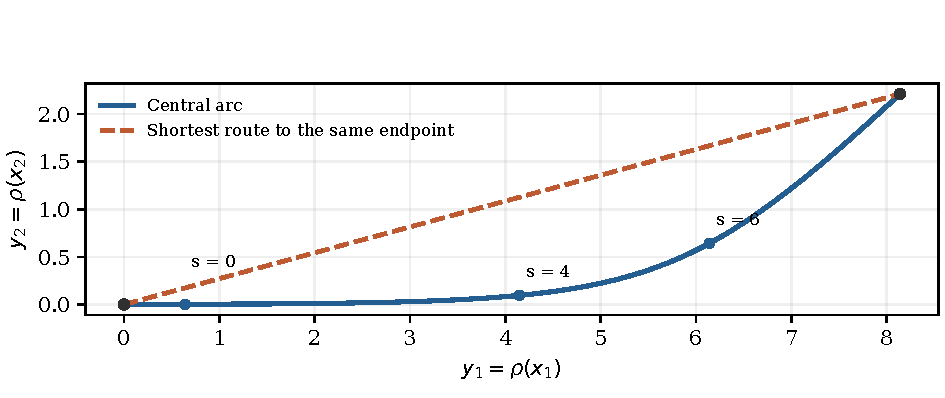
\includegraphics[width=.82\textwidth]{figures/flattened-path.pdf}
 \caption{A two-coordinate example in the exact metric coordinates
 $y_i=\rho(x_i)$. The barrier is $b(x_1)+b(x_2)$, objective weights are
 $(1,e^{-6})$, and the terminal logarithmic parameter is $s=8$.
 The central arc starts at the analytic-center limit $s=-\infty$.
 The straight segment is a globally shortest route to the same endpoint.
 The plot illustrates endpoint geometry; it does not display the closest
 point in an objective target set.}
 \label{fig:flattened}
\end{figure}

Our main results develop this mechanism in four directions.
\begin{enumerate}[leftmargin=*,label=\arabic*.]
\item \emph{Exact spectral geometry and the sharp rank factor.}
For rectangular real or complex spectral-norm balls and spectral
intervals in every Euclidean Jordan algebra, equipped with their standard
log-determinant barriers, distance from the analytic center is exactly
the Euclidean norm of the transformed singular values
or eigenvalues. Leaving the objective's spectral frame cannot shorten
this route. Distance to the entire accurate target set reduces to a
strictly convex scalar allocation with one multiplier
(\cref{thm:exact-distance,thm:water-filling}).
For equal barrier scales and $r$ active objective channels, every central
subarc satisfies
\begin{equation}
 L_{\CP}\leq\Gamma_r d_F(\text{its endpoints}),\qquad
 \Gamma_r=\left[\sum_{i=1}^r(\sqrt i-\sqrt{i-1})^2\right]^{1/2},
 \qquad \Gamma_r^2=\tfrac14\log r+O(1).
 \label{eq:intro-Gamma}
\end{equation}
The supremum of this ratio is exactly $\Gamma_r$.
For the same objective accuracy,
$L_{\CP}(\eps)\leq c_\star\Gamma_r L_\opt(\eps)$,
where $1.37486<c_\star<1.38$ is the sharp constant in a specified scalar
KKT comparison, certified by rational arithmetic. Sharpness of the
product $c_\star\Gamma_r$ is not asserted
(\cref{thm:sharp-prefix,thm:scalar-dilation}).
Unequal factor scales give an exact weighted prefix constant; its value
depends on activation order and can have order $\sqrt r$ when the scale
range grows exponentially (\cref{prop:scale-order}).

\item \emph{A separation for actual finite sequences.}
An explicit dyadic objective and tolerance on the cube give
$L_\opt=\Theta(r\sqrt{\log r})$ and
$L_\CP=\Theta(r\log r)$, with ordinary input length
$\Theta(r^2)$ (\cref{thm:dyadic}). A clipped progress function proves
that every forward-$R$ sequence in a fixed metric tube around the
central path needs $\Omega(r\log r)$ moves to attain actual accuracy,
with a matching $O(r\log r)$ construction.
The labels may be arbitrary and nonmonotone; no sampling assumption is
imposed on the competing sequence. More generally, a diverging overhead
survives tube radii $\delta_r=o((\log r)^{1/3})$
(\cref{thm:tube}). Fixed Newton-decrement neighborhoods of radius
$0\leq\beta<1/2$ satisfy this contract. The distinction between central arclength and finite sequences
is necessary: an arclength lower bound alone does not exclude chords
that skip a long part of a curve.

\item \emph{Persistence beyond the standard separable barrier.}
Every fixed scalar barrier satisfying the positive-branch normalization
$(f')^2\leq f''$ has the same sharp endpoint factor $\Gamma_r$,
a uniform same-accuracy comparison with constant $C_{\SC}<2$, and the
same dyadic separation. This includes the universal and entropic cube
barriers (\cref{thm:normalized-scalar,prop:canonical-cube}).
The scalar normalization has content: the unrestricted class admits
ratios approaching $\sqrt r$, with a growing scalar parameter.
Convex couplings with bounded first and second derivatives on one full
facet collar retain a worst ratio at least $\Gamma_r$
(\cref{thm:facet-coupling}). We give dense and fully signed-permutation
invariant coupled examples with exact, optimal cube parameter $r$.
For the explicit radial family
\[
 F_{\lambda,c}(x)=U(x)-\lambda\log(c-\norm x^2),
 \qquad \lambda\geq1,\quad c-r\geq4\lambda,
\]
we also prove a matching $O(\Gamma_r)$ upper comparison and uniform
persistence of the finite-sequence separation, even when $\lambda,c$
vary with dimension (\cref{thm:radial-upper,cor:radial-discrete}).
Thus optimal parameter and substantial symmetry do not ensure a bounded
centrality ratio. The matching upper theorem concerns this explicit
family; the facet-collar theorem for general couplings is a lower bound.

\item \emph{The additional cost of a dual completion.}
Classical primal--dual geometry fixes total central speed at $\sqrt\nu$
in logarithmic parameter. We calculate how objective activity divides
this speed between primal and dual components. An optimal product-ball
cone barrier permits much less primal movement than its parameter alone
would suggest, even with positive weights and a unique projected
optimizer. Most directly, the same dyadic sparse LP has optimal primal
movement $\Theta(r\sqrt{\log r})$, central primal movement
$\Theta(r\log r)$, and movement to any feasible full small-gap point
$\Theta(r^{3/2})$ (\cref{thm:completion}). The metric and endpoint
contracts are stated separately in that theorem.
\end{enumerate}

The supporting results identify when these comparisons survive additional
structure. Effective objective rank gives explicit velocity and error
laws, including geometric and polynomial spectral decay; a determinant
rank certificate can miss an unbounded target distance
(\cref{sec:distribution}). For changes of formulation, an exposed
Jordan minor gives a weighted support-rank lower bound that allows all
auxiliary fibers to move. A dimension cap on operational cone factors
gives a full primal--dual lower bound for arbitrary logarithmically
homogeneous barriers. Grouped balls, norm trees and arbitrary PSD column
packing provide complete fixed-metric examples, including exact restricted
parameters and heterogeneous objective scales
(\cref{sec:formulation,app:formulations}). These consequences distinguish
which information comes from the objective, the barrier, and the lift.

\subsection{Relationship to prior work}
\label{subsec:geometric-prior}

Nesterov and Todd~\cite{NesterovTodd2002} established the basic
Riemannian geometry of self-concordant barriers, its connection to bounded
local steps, and the product rule for distances. Their Section~6.2
flattens a separable hypercube metric by integrating its scalar local
norm. Their primal--dual theorem bounds central length by $\sqrt2$ times
endpoint distance in the metric of a logarithmically homogeneous cone
barrier plus its conjugate. Their Theorem~5.1(c) and Corollary~5.1 already
extend the comparison to the entire feasible small-gap set, with possible
affine infeasibility at intermediate points. We restate this classical
result in \cref{thm:pd-gap-set} to make the contrast with primal shortcuts
precise; the gap-set extension is not an original contribution.

Nesterov and Nemirovski~\cite{NesterovNemirovski2008} studied primal
central paths versus geodesics. If $D$ is the distance between two
central points, their Theorem~4.1 gives
\begin{equation}
 L\leq\log2+\nu^{1/4}\sqrt{D(D+\log12)}.
 \label{eq:NN-comparison}
\end{equation}
Their Example~1.1 distinguishes a central endpoint from an objective
target set, and their Theorem~5.3 gives a target-set comparison under
an explicit separation assumption. The present work addresses that
established comparison problem on specified spectral domains: it
computes the accurate-target benchmark and replaces the general
parameter dependence by an exact active-rank constant for these metrics.

Worst-case central-path behavior and lower bounds for path-following
methods have a substantial separate history. Deza, Nematollahi and
Terlaky~\cite{DezaNematollahiTerlaky2008} study iteration lower bounds
through Klee--Minty constructions. Allamigeon, Benchimol, Gaubert and
Joswig~\cite{AllamigeonEtAl2018} construct long-winding logarithmic
central paths and prove exponential neighborhood iteration lower bounds.
Allamigeon, Gaubert and
Vandame~\cite{AllamigeonGaubertVandame2022} give exponential lower bounds
for self-concordant-barrier path-following methods in their prescribed
neighborhood model. Allamigeon, Dadush, Loho, Natura and
V\'egh~\cite{AllamigeonEtAl2025} compare an interior-point method with
\emph{straight-line complexity}, which counts affine segments in a wide
central neighborhood, and obtain comparisons across self-concordant
barriers. Dadush, Ma, Natura and V\'egh~\cite{DadushMaNaturaVegh2026}
improve wide-neighborhood guarantees expressed in terms of straight-line
complexity and establish approximate instance optimality of trust-region
path following in the narrow $\ell_2$ neighborhood. Their affine-segment
and algorithmic iteration resources differ from the fixed-radius
local-Hessian moves counted here. Our dyadic example gives a separation between
central-neighborhood movement and unrestricted target distance in the
same metric on the same simple domain; it is not a first demonstration
of central-path inefficiency or a barrier-independent exponential
iteration lower bound.

Several ingredients have direct classical antecedents. The prefix norm
inequality is a finite weighted Lorentz-norm inequality
\cite{Lorentz1951}; the new comparison requires its sharp realization by
translated central velocities. The matrix and Jordan Hessian calculations
use spectral differentiation~\cite{LewisSendov2001,Baes2007}.
Metric projections and conjugate Hessian isometries appear explicitly
in Ohara, Ishi and Tsuchiya~\cite{OharaIshiTsuchiya2024}.
The universal and entropic constructions and their exact dimension
parameters are due to earlier work
\cite{NesterovNemirovskii1994,LeeYue2021,BubeckEldan2019,Chewi2023};
we derive their centrality consequences. Parameter-preserving diagonal
quadratic regularization on boxes is also prior work
\cite{CastroCuesta2011}. The coupled examples here supplement that
construction literature with exact-parameter path comparisons.

Geodesic updates in symmetric-cone algorithms
\cite{Permenter2023} and interior-point methods on Riemannian base
manifolds~\cite{HiraiNieuwboerWalter2026} concern complementary algorithmic
settings. The real Hessian metric on a bounded spectral ball used here
is distinct from the affine-invariant metric on a symmetric cone and
from complex Bergman metrics. The formulas are proved for the stated
metric, including complex matrix spaces viewed as real vector spaces.

To the best of our knowledge, the exact active-rank supremum
\eqref{eq:intro-Gamma} for these central paths, its combination with the
explicit accurate-target allocation, the dyadic finite-sequence
separation with arbitrary labels, the uniform comparison for the stated
radial coupled family, and the same-instance three-scale completion
comparison have not appeared in the cited literature. These are the
specific original claims supported by our proofs and literature review.
The general geometric framework, canonical barriers, and classical
primal--dual gap-set comparison are antecedents of these results.

\subsection{Organization}
\Cref{sec:foundations} fixes the metric and local-step conventions.
\Cref{sec:exact-distance,sec:sharp-centrality} establish the exact
benchmark and sharp comparison; \cref{sec:distribution,sec:discrete}
develop objective profiles and finite sequences.
\Cref{sec:barrier-dependence,sec:coupled-barriers} treat scalar and
coupled changes of barrier. \Cref{sec:primal-dual,sec:formulation}
separate dual completion from formulation effects.
The appendices give the rational scalar certificate, the normalized
profile envelope and nonmonotone construction, and the complete proofs
for the concrete formulations. The figures are reproducible numerical
illustrations of analytically proved results.

\section{Barrier geometry and the comparison problem}
\label{sec:foundations}

The paper makes three different comparisons: a central arc with the
shortest path to the same endpoint; a central arc with the shortest path
to any point that is at least as accurate; and primal movement with the
movement of a feasible primal--dual pair. Each statement specifies its
set of endpoints and its metric.

\subsection{Definitions and step counts}
Let $\Omega$ be an open convex subset of a finite-dimensional real inner
product space $E$. A $C^3$ function $F:\Omega\to\R$ with positive definite
Hessian defines a local norm, curve length, and distance:
\begin{equation}
 \norm{h}_{F,x}^2=D^2F(x)[h,h],\qquad
 \Len_F(\gamma)=\int_0^1\norm{\dot\gamma(t)}_{F,\gamma(t)}\dd t,
 \qquad
 d_F(x,y)=\inf_{\gamma:x\leadsto y}\Len_F(\gamma).
 \label{eq:metric-definitions}
\end{equation}
The infimum is over absolutely continuous curves in $\Omega$.
On an affine slice of $\Omega$, norms are restricted to the tangent
space of the slice, and curves stay in the slice. Complex matrix
spaces are treated as real vector spaces, with inner product $\operatorname{Re}\tr(X^*Y)$.

We call $F$ a standard self-concordant barrier if it tends to $+\infty$
at every finite boundary point and satisfies
\begin{equation}
 \abs{D^3F(x)[h,h,h]}\leq2\norm{h}_{F,x}^3.
 \label{eq:self-concordance}
\end{equation}
Its barrier parameter is any $\nu$ satisfying
$\abs{DF(x)[h]}\leq\sqrt\nu\norm{h}_{F,x}$ for all $x,h$; the least
such $\nu$ is the exact parameter.
In ``standard self-concordant'', the word ``standard'' refers to the
constant $2$ in \eqref{eq:self-concordance}; ``the standard barriers''
means the logarithmic and log-determinant barriers of
\cref{sec:exact-distance} and their products, with any positive scales.
They are standard self-concordant when every scale is at least one
(\cref{prop:standard-parameters}).
Self-concordance implies the polarized inequality
\begin{equation}
 \abs{D^3F(x)[u,h,h]}\leq2\norm{u}_{F,x}\norm{h}_{F,x}^2.
 \label{eq:mixed-SC}
\end{equation}
We write $\norm{h}_x$ when $F$ is fixed.

\begin{lemma}[Distance and the local norm of a chord]
\label{lem:chord-distance}
For a standard self-concordant barrier,
\begin{equation}
 \log(1+\norm{y-x}_x)\leq d_F(x,y).
 \label{eq:global-chord}
\end{equation}
If $q=\norm{y-x}_x<1$, the straight segment from $x$ to $y$ has length
at most $-\log(1-q)$. In particular, for $0<R<1$,
\begin{equation}
 \norm{y-x}_x\leq R\ \Longrightarrow\ d_F(x,y)\leq-\log(1-R),
 \qquad
 d_F(x,y)\leq\log(1+R)\ \Longrightarrow\ \norm{y-x}_x\leq R.
 \label{eq:two-chord-bounds}
\end{equation}
\end{lemma}
\begin{proof}
Along any curve $\gamma$ starting at $x$, let
$\ell(t)=\int_0^t\norm{\dot\gamma(u)}_{\gamma(u)}\dd u$.
For a fixed vector $h\ne0$, \eqref{eq:mixed-SC} gives
$\abs{\frac{\mathrm d}{\mathrm dt}\log\norm{h}_{\gamma(t)}}
\leq\dot\ell(t)$ almost everywhere. Thus
$\norm{h}_x\leq e^{\ell(t)}\norm{h}_{\gamma(t)}$ for every $h$.
The triangle inequality in the fixed norm at $x$ now gives
\[
 \norm{y-x}_x\leq\int_0^1\norm{\dot\gamma(t)}_x\dd t
 \leq\int_0^1e^{\ell(t)}\dot\ell(t)\dd t=e^{\Len_F(\gamma)}-1.
\]
Taking the infimum proves \eqref{eq:global-chord}.
For the segment $x+th$, $h=y-x$, set $a(t)=\norm{h}_{x+th}$.
Self-concordance gives $\abs{a'(t)}\leq a(t)^2$ and hence
$a(t)\leq q/(1-tq)$ while $tq<1$. Integration from $0$ to $1$ gives
the second assertion. The segment lies in $\Omega$ by convexity.
\end{proof}

These estimates underlie the short-step counts of Nesterov and
Todd~\cite[Section~3]{NesterovTodd2002}.
For a target set $A\subset\Omega$ and a starting point $x_0$, let
$D_F(x_0,A)=\inf_{x\in A}d_F(x_0,x)$.
A forward-$R$ sequence is a finite sequence $x_0,x_1,\ldots,x_T$ of
points in $\Omega$ such that $\norm{x_{j+1}-x_j}_{x_j}\leq R$; its $T$
steps are called forward $R$-chords.

\begin{corollary}[Optimal bounded movement]
\label{cor:optimal-movement}
Let $F$ be a standard self-concordant barrier and $0<R<1$.
Every forward-$R$ sequence from $x_0$ to $A$ satisfies
\begin{equation}
 T\geq\frac{D_F(x_0,A)}{-\log(1-R)}.
 \label{eq:movement-lower}
\end{equation}
If a shortest curve to $A$ exists, there is such a sequence with
\begin{equation}
 T\leq\left\lceil\frac{D_F(x_0,A)}{\log(1+R)}\right\rceil.
 \label{eq:movement-upper}
\end{equation}
\end{corollary}
\begin{proof}
For the lower bound, join consecutive points by straight segments and
apply \cref{lem:chord-distance}. For the upper bound, divide a shortest
curve into arcs of length at most $\log(1+R)$ and apply
\eqref{eq:global-chord} to their endpoints. If the distance is zero and
attained, no step is needed.
\end{proof}

For a bounded domain and a nonzero objective vector $c\in E$, define the
support value, the objective gap, and the $\eps$-accurate set:
\begin{equation}
 h_\Omega(c)=\sup_{x\in\Omega}\ip{c}{x},\qquad
 g_c(x)=h_\Omega(c)-\ip{c}{x},\qquad
 A_\eps=\{x\in\Omega:g_c(x)\leq\eps\}.
 \label{eq:gap-target}
\end{equation}
When $F$ is a strictly convex barrier, the central point with parameter
$\eta$ is
\begin{equation}
 x(\eta)=\argmin_{x\in\Omega}\{F(x)-\eta\ip{c}{x}\},\qquad \eta\geq0.
 \label{eq:central-path}
\end{equation}
At $\eta=0$ it is the analytic center $x_0$.
We write $L_\opt(\eps)=D_F(x_0,A_\eps)$ and
$L_\CP(\eta)=\Len_F(x|_{[0,\eta]})$; $L_\CP(\eta_0,\eta_1)$ is the
length of the arc between parameters $\eta_0$ and $\eta_1$, and
$L_\CP(\eps)=L_\CP(\eta_\eps)$, where $\eta_\eps$ is the first
parameter with $g_c(x(\eta_\eps))=\eps$. We say whether the argument
of $L_\CP$ is a parameter or an accuracy whenever this is ambiguous.

\section{Exact distance and the closest accurate endpoint}
\label{sec:exact-distance}

A single scalar coordinate describes all the metrics in this section.
Let
\begin{equation}
 b(t)=-\log(1-t^2),\qquad
 \rho(t)=\int_0^t\frac{\sqrt{2(1+u^2)}}{1-u^2}\dd u,
 \qquad -1<t<1.
 \label{eq:rho-def}
\end{equation}
Then $\rho$ is odd, strictly increasing, maps $(-1,1)$ onto $\R$, and
$\rho'(t)^2=b''(t)$. For $0\leq t<1$,
\begin{equation}
 \log\frac1{1-t}\leq\rho(t)\leq\sqrt2\log\frac1{1-t}.
 \label{eq:rho-log}
\end{equation}
Indeed, after multiplying the corresponding derivative inequalities by
$1-t$, these bounds reduce to
$1\leq\sqrt{2(1+t^2)}/(1+t)\leq\sqrt2$.

\subsection{Boxes, rectangular matrix balls, and Jordan intervals}
For a box $(-1,1)^n$ with $F(x)=\sum_i\alpha_i b(x_i)$,
$\alpha_i>0$, integration of the diagonal metric gives
\begin{equation}
 d_F(x,y)^2=\sum_i\alpha_i\bigl(\rho(x_i)-\rho(y_i)\bigr)^2.
 \label{eq:box-distance}
\end{equation}
The transformed straight segment stays in the box and attains this
distance. This scalar product construction is classical; the point of
the next theorem is that leaving a spectral frame cannot shorten the
route from the center.

For $\F\in\{\R,\C\}$ and $p\leq q$, put
\begin{equation}
 \ball_{p,q}^{\F}=\{X\in\F^{p\times q}:\norm{X}_{\op}<1\},\qquad
 \Phi_\alpha(X)=-\alpha\log\det(I_p-XX^*),\quad \alpha>0.
 \label{eq:matrix-ball}
\end{equation}
Write $\sigma^\downarrow(X)$ for its $p$ singular values, in decreasing
order, including zeros.

We also use a Euclidean Jordan algebra $V$, of rank $n$, with unit $e$,
cone of squares $K$, Jordan product $x\circ y$, and trace inner product
$\ip{x}{y}=\tr(x\circ y)$. A Jordan frame $(e_i)_{i=1}^n$ consists of
orthogonal primitive idempotents with sum $e$. The spectral theorem gives
$x=\sum_i\lambda_i(x)e_i$ and $\det x=\prod_i\lambda_i(x)$.
A primitive idempotent is a nonzero element $u$ with $u\circ u=u$
that cannot be written as the sum of two nonzero orthogonal idempotents.
The spectral interval and its barrier are
\begin{equation}
 \mathcal I(V)=\{x:-e\prec_Kx\prec_Ke\},\qquad
 \Phi_\alpha(x)=-\alpha\log\det(e-x^2)
 =\alpha\sum_{i=1}^n b(\lambda_i(x)).
 \label{eq:jordan-interval}
\end{equation}
Here $x^2=x\circ x$ and $u\prec_Kv$ means $v-u\in\interior K$.
The examples include real, complex, and quaternionic Hermitian matrices,
Lorentz algebras, their direct products, and the exceptional Albert
algebra. Rank, rather than the real dimension of $V$, counts the spectral
coordinates.

\begin{theorem}[Exact spectral distance]
\label{thm:exact-distance}
For every $\alpha>0$, the following identities hold:
\begin{align}
 d_{\Phi_\alpha}(0,X)^2
   &=\alpha\sum_{i=1}^p\rho(\sigma_i(X))^2,
   &&X\in\ball_{p,q}^{\F}, \label{eq:matrix-radial-distance}\\
 d_{\Phi_\alpha}(0,x)^2
   &=\alpha\sum_{i=1}^n\rho(\lambda_i(x))^2,
   &&x\in\mathcal I(V). \label{eq:jordan-radial-distance}
\end{align}
More generally,
\begin{align}
 d_{\Phi_\alpha}(X,Y)
 &\geq\sqrt\alpha\,
 \norm{\rho(\sigma^\downarrow(X))-\rho(\sigma^\downarrow(Y))}_2,
 \label{eq:matrix-contraction}\\
 d_{\Phi_\alpha}(x,y)
 &\geq\sqrt\alpha\,
 \norm{\rho(\lambda^\downarrow(x))-\rho(\lambda^\downarrow(y))}_2.
 \label{eq:jordan-contraction}
\end{align}
Here $\rho$ acts coordinatewise and the Jordan eigenvalues are ordered
by signed value. Equality holds in each contraction when the two
endpoints have a common ordered spectral frame. The minimizing path is
linear in the $\rho$ coordinates of that frame.
\end{theorem}
\begin{proof}
First consider matrices. Introduce the Hermitian dilation and a scalar
function
\[
 S(X)=\begin{pmatrix}0&X\\X^*&0\end{pmatrix},\qquad
 g(t)=-\tfrac12\log(1-t^2).
\]
The eigenvalues of $S(X)$ are $\pm\sigma_i(X)$ and $q-p$ zeros, so
$\Phi_\alpha(X)=\alpha\tr g(S(X))$. In an eigenbasis of a Hermitian
matrix $S$ with eigenvalues $\lambda_a$, the spectral-trace Hessian is
\begin{equation}
 D^2\tr g(S)[H,H]
 =\sum_a g''(\lambda_a)|H_{aa}|^2
 +2\sum_{a<b}\frac{g'(\lambda_a)-g'(\lambda_b)}{\lambda_a-\lambda_b}
       |H_{ab}|^2.
 \label{eq:hermitian-Hessian}
\end{equation}
The quotient at equal eigenvalues means $g''(\lambda_a)$.
For completeness, the gradient of $\tr g(S)$ is $g'(S)$.
Differentiating a polynomial in $S$ shows that the $(a,b)$ entry of
$Dg'(S)[H]$ is the displayed divided difference times $H_{ab}$.
The convergent power series of $g$ on $(-1,1)$ justifies the same
calculation here, uniformly on compact spectral subintervals.
Taking its inner product with $H$ gives
\eqref{eq:hermitian-Hessian}, over the real and complex fields alike.
This is the trace-separable case of the spectral Hessian
formula~\cite{LewisSendov2001}.

All divided differences in \eqref{eq:hermitian-Hessian} are positive.
The ordered eigenvalues of an absolutely continuous Hermitian path are
absolutely continuous; almost everywhere their derivatives are the
eigenvalues of the derivative compressed to each repeated eigenspace.
Thus one can choose the eigenbasis within each such space to identify
the diagonal contributions with these derivatives. Applying the formula
to $S(X(t))$ gives
\begin{equation}
 \norm{\dot X(t)}_{\Phi_\alpha,X(t)}^2
 \geq\alpha\sum_i b''(\sigma_i(X(t)))\dot\sigma_i(X(t))^2
 =\alpha\norm{\tfrac{\mathrm d}{\mathrm dt}\rho(\sigma(X(t)))}_2^2
 \quad\text{a.e.}
 \label{eq:singular-speed-contraction}
\end{equation}
The factor is $b''$, because each pair contributes $2g''=b''$.
Singular values are Lipschitz functions of the matrix, and at zero or
repeated singular values the same almost-everywhere rule follows from
the dilation. Integration proves \eqref{eq:matrix-contraction}.
For a fixed singular value decomposition $X=U\diag(\sigma_i)V^*$,
the path
\begin{equation}
 X(t)=U\diag\bigl(\rho^{-1}(t\rho(\sigma_i))\bigr)V^*,
 \qquad 0\leq t\leq1,
 \label{eq:radial-geodesic}
\end{equation}
has constant speed equal to the right side of
\eqref{eq:matrix-radial-distance} to the power $1/2$.
Indeed, restricting $\Phi_\alpha$ to this frame gives
$\alpha\sum_i b(x_i)$. The lower bound therefore is attained.
Interpolation between two coordered transformed spectra gives the other
equality assertion; order is preserved under this interpolation.

Here are the details for Jordan algebras. Relative to a Jordan frame, the
Peirce spaces are $V_{ii}=\R e_i$ and, for $i<j$,
\[
 V_{ij}=\{h:e_i\circ h=e_j\circ h=\tfrac12h,
                  \ e_k\circ h=0\text{ for }k\notin\{i,j\}\}.
\]
At $x=\sum_i\lambda_i e_i$, write the orthogonal Peirce decomposition
of a vector $h$ as $h=\sum_i h_i e_i+\sum_{i<j}h_{ij}$, where
$h_{ij}\in V_{ij}$ and $\norm{e_i}=1$. The Hessian is
\begin{equation}
 D^2\Phi_\alpha(x)[h,h]
 =\alpha\sum_i b''(\lambda_i)h_i^2
 +\alpha\sum_{i<j}
 \frac{b'(\lambda_i)-b'(\lambda_j)}{\lambda_i-\lambda_j}
       \norm{h_{ij}}^2.
 \label{eq:jordan-Hessian}
\end{equation}
One way to verify this formula without restricting the algebra type is
to differentiate the gradient
$\alpha((e-x)^{-1}-(e+x)^{-1})$.
To compute the derivative of inversion at a positive diagonal element
$z=\sum_i z_i e_i$, let $L_z h=z\circ h$ and differentiate
$z\circ z^{-1}=e$. This gives
$L_z D(z^{-1})[h]=-L_{z^{-1}}h$.
The operator $L_z$ is positive definite: it acts by $z_i$ on $V_{ii}$
and by $(z_i+z_j)/2$ on $V_{ij}$.
On the same spaces, $L_{z^{-1}}$ acts by $z_i^{-1}$ and
$(z_i^{-1}+z_j^{-1})/2$, respectively. Solving the differentiated
identity therefore gives the inversion coefficients $-z_i^{-2}$ and
$-(z_i z_j)^{-1}$. The resulting off-diagonal coefficient is
\[
 \frac1{(1-\lambda_i)(1-\lambda_j)}
 +\frac1{(1+\lambda_i)(1+\lambda_j)}
 =\frac{b'(\lambda_i)-b'(\lambda_j)}{\lambda_i-\lambda_j}.
\]
This also gives its continuous value at a repeated eigenvalue.
Every coefficient is positive. Jordan eigenvalues obey the same local
Lipschitz and repeated-eigenspace derivative rule: within the Peirce
algebra for a repeated eigenvalue, diagonalize the corresponding
component of $h$. Equivalently, this follows from the spectral variational
principle applied to $x+th$. Hence, along an absolutely continuous curve,
\[
 \norm{\dot x}_{\Phi_\alpha,x}^2
 \geq\alpha\sum_i b''(\lambda_i(x))\dot\lambda_i(x)^2.
\]
Integrate and interpolate in a fixed Jordan frame exactly as above.
Only the Jordan spectral theorem and Peirce rules have been used, so
the argument includes the exceptional algebra.
\end{proof}

The scale condition in the theorem is only $\alpha>0$, since distance
uses the Hessian. The local-step conclusions need self-concordance.

\begin{proposition}[Self-concordance and parameter]
\label{prop:standard-parameters}
If $\alpha\geq1$, the barriers in \eqref{eq:matrix-ball} and
\eqref{eq:jordan-interval} are standard self-concordant barriers.
Their least gradient parameters are respectively $\alpha p$ and
$\alpha n$. A product with scales $\alpha_j\geq1$ has least gradient
parameter equal to the sum of these parameters.
\end{proposition}
\begin{proof}
The matrix barrier at scale one is the restriction of the positive
Hermitian log-determinant barrier to
$\left(\begin{smallmatrix}I_p&X\\X^*&I_q\end{smallmatrix}\right)$.
The Jordan barrier is the restriction of
$-\log\det u-\log\det v$ to $(u,v)=(e-x,e+x)$.
The log-determinant is self-concordant: after its Hessian isometry at an
interior point, the second and third directional derivatives are
$\sum_i\xi_i^2$ and $-2\sum_i\xi_i^3$, so
$|\sum_i\xi_i^3|\leq(\sum_i\xi_i^2)^{3/2}$.
Affine restriction and addition preserve self-concordance, as does
multiplication by $\alpha\geq1$. Boundary divergence follows from the
vanishing determinant.

The gradient has no component outside the spectral frame, and the
Hessian has no mixed term between that frame and its orthogonal
complement. Thus its squared dual norm is
\begin{equation}
 \norm{\nabla\Phi_\alpha}_{\Phi_\alpha,*}^2
 =\alpha\sum_i\frac{b'(t_i)^2}{b''(t_i)}
 =\alpha\sum_i\frac{2t_i^2}{1+t_i^2}
 <\alpha n_0,
 \label{eq:exact-standard-parameter}
\end{equation}
where $n_0=p$ and $t_i=\sigma_i$ for a matrix ball, and $n_0=n$ and
$t_i=\lambda_i$ for a Jordan interval. In the matrix case this block
structure follows either from \eqref{eq:hermitian-Hessian} or by
differentiating the invariant trace function in singular coordinates.
Letting all $t_i$ tend to $1$ proves that the supremum is $\alpha n_0$.
For products, squared gradient dual norms add, and the limits can be
approached simultaneously.
\end{proof}

\subsection{Distance to an objective target set}
\label{subsec:water-filling}
Consider any finite product of the domains just defined. Each factor
has its own scale $\alpha_j>0$. A nonzero support objective has active
weights $w_i>0$: the positive singular values of each matrix objective,
or the absolute values of the nonzero Jordan eigenvalues of each Jordan
objective. Pool all these weights, indexed by $1\leq i\leq r$, and
attach to each its factor's scale $\alpha_i$. Within a factor all scales
are therefore equal. For a scalar box this simply means
$w_i=|c_i|$ at the nonzero coordinates. Let $W_0=\sum_i w_i$; the
support value is $W_0$ and the analytic center is zero.

\begin{theorem}[The closest accurate endpoint]
\label{thm:water-filling}
For $0<\eps<W_0$, the distance to the entire objective target set is
\begin{equation}
 L_\opt(\eps)^2
 =\min\left\{\sum_{i=1}^r\alpha_i\rho(x_i)^2:
      0\leq x_i<1,\quad\sum_{i=1}^r w_i(1-x_i)\leq\eps\right\}.
 \label{eq:water-filling}
\end{equation}
The scalar allocation problem has a unique minimizer, all coordinates
lie in $(0,1)$, and its constraint is active. There is a unique
$\lambda>0$ such that
\begin{equation}
 2\alpha_i\rho(x_i)\rho'(x_i)=\lambda w_i\quad(1\leq i\leq r),
 \qquad \sum_iw_i(1-x_i)=\eps.
 \label{eq:water-KKT}
\end{equation}
An aligned endpoint with these coordinates and all inactive coordinates
zero attains the minimum distance in the original domain. The path
linear in its transformed spectral coordinates is globally shortest
to the target set.
\end{theorem}
\begin{proof}
Distances in a product metric add in squares. To see this directly, the
length of a product curve is the integral of the Euclidean norm of its
component speeds, which is at least the Euclidean norm of the component
lengths. Constant-speed shortest component curves attain equality; such
curves from zero were constructed in \cref{thm:exact-distance}.

For a matrix factor, von Neumann's trace inequality gives
$\ip{C}{X}\leq\sum_iw_i\sigma_i(X)$, with weights and singular values
ordered. Thus replacing an endpoint by one in the objective's singular
frame can only improve its objective and leaves its distance unchanged.
Inactive singular values can then be set to zero, reducing the distance.
For a Jordan factor, if $(e_i)$ and $(f_j)$ are frames of $c$ and $x$,
the entries $m_{ij}=\ip{e_i}{f_j}$ are nonnegative and their row and
column sums are one. Therefore
\[
 \ip{c}{x}=\sum_{i,j}\mu_i\lambda_j m_{ij}
 \leq\sum_i|\mu|_i^\downarrow|\lambda|_i^\downarrow.
\]
The last inequality is the rearrangement inequality for a doubly
stochastic matrix. Assigning magnitudes to the objective frame in this
order and using the signs of $\mu_i$ attains the bound, at the same
radial distance. Zero-weight coordinates can again be removed.
Conversely every scalar vector in \eqref{eq:water-filling} gives an
aligned feasible endpoint with precisely that objective error and
radial distance. This proves the reduction.

For $x\geq0$, $\rho'>0$, $\rho''\geq0$, and
$(\rho^2)''=2((\rho')^2+\rho\rho'')>0$.
The objective is therefore strictly convex. It tends to infinity if
any coordinate tends to $1$. A nonempty bounded sublevel set is compact
in $[0,1)^r$, so a minimizer exists and is unique.
Its accuracy constraint must be active: otherwise reduce one positive
coordinate slightly. Slater's condition holds by taking every
coordinate sufficiently close to $1$. The KKT multiplier is positive,
since a zero multiplier would force every coordinate to be zero, which
violates $\eps<W_0$. At $x_i=0$ the objective's derivative is zero,
whereas the accuracy constraint contributes $-\lambda w_i<0$;
stationarity with a nonnegative multiplier for $-x_i\leq0$ is then
impossible. Every coordinate is positive, and stationarity gives
\eqref{eq:water-KKT}.

The function $(\rho^2)'$ increases continuously from zero to infinity.
For a fixed $\lambda>0$, each equation in \eqref{eq:water-KKT} thus has
one solution. Their weighted residual decreases continuously and
strictly from $W_0$ to zero as $\lambda$ increases from zero to infinity.
This proves uniqueness of $\lambda$ and supplies a scalar search.
The minimizing path follows from \cref{thm:exact-distance} and the
product rule. Within each factor the minimizer is ordered with its
weights because its scales agree, so the common-frame construction
applies without an ordering issue.
\end{proof}

The uniqueness assertion concerns the scalar allocation. It is not
needed to assert uniqueness of all ambient matrix representations at
repeated objective eigenvalues. If $\eps\geq W_0$, the analytic center
has zero cost. For $\eps=0$, no strictly interior point is accurate, and
$L_\opt(\eps)\to\infty$ as $\eps\downarrow0$.

\begin{corollary}[Logarithmic allocation and bounded moves]
\label{cor:water-movement}
Let $0<\eps<W_0$. Define
\begin{equation}
 D_{\log}(\eps)^2=
 \min\left\{\sum_i\alpha_i s_i^2:s_i\geq0,
                    \quad\sum_i w_i e^{-s_i}\leq\eps\right\}.
 \label{eq:log-water-filling}
\end{equation}
Then
\begin{equation}
 D_{\log}(\eps)\leq L_\opt(\eps)\leq\sqrt2D_{\log}(\eps).
 \label{eq:log-comparison}
\end{equation}
Its unique optimizer satisfies
\begin{equation}
 s_i=\mathcal W(\gamma w_i/\alpha_i),\qquad
 \sum_i\alpha_i\mathcal W(\gamma w_i/\alpha_i)=\gamma\eps,
 \quad\gamma>0,
 \label{eq:Lambert}
\end{equation}
where $\mathcal W$ is the nonnegative inverse of $s\mapsto s e^s$.
For $0<R<1$, if all scales are at least one, the minimum number
$T_R^\star(\eps)$
of feasible forward-$R$ moves from zero to any accurate endpoint obeys
\begin{equation}
 \frac{L_\opt(\eps)}{-\log(1-R)}
 \leq T_R^\star(\eps)
 \leq\left\lceil\frac{L_\opt(\eps)}{\log(1+R)}\right\rceil.
 \label{eq:exact-bounded-movement}
\end{equation}
\end{corollary}
\begin{proof}
Set $s_i=-\log(1-x_i)$ and apply \eqref{eq:rho-log} to every feasible
allocation. Strict convexity and the KKT conditions for
\eqref{eq:log-water-filling} give
$\alpha_i s_i=\gamma w_i e^{-s_i}$ with all $s_i>0$.
Inverting and summing these identities gives \eqref{eq:Lambert}.
Uniqueness follows, for example, by observing that
$\sum_iw_i\exp[-\mathcal W(\gamma w_i/\alpha_i)]$ decreases strictly
from $W_0$ to zero; the zero root of the multiplied equation in
\eqref{eq:Lambert} is excluded by $\gamma>0$.
Finally, \cref{prop:standard-parameters,cor:optimal-movement} apply,
and the shortest curve was constructed in \cref{thm:water-filling}.
\end{proof}

The construction is explicit once the objective frame is available.
Invert $(\rho^2)'$ coordinatewise and use doubling and bisection for the
positive multiplier. An upper bracket whose residual is at most the
requested tolerance gives an accurate endpoint. Along the resulting
path, checkpoints at arc intervals $\log(1+R)$ satisfy the forward
local-norm restriction. Finite-precision evaluation must preserve these
two inequalities, for instance by using strict accuracy and step-radius
margins. We make no arithmetic-complexity claim for this scalar search
or for obtaining the spectral frame.

\section{Sharp comparison for the standard spectral barriers}
\label{sec:sharp-centrality}
The reduction in \cref{thm:water-filling} applies to all products considered
there. An active channel means a positive singular value of a matrix
objective, or the absolute value of a nonzero Jordan eigenvalue. Denote
these weights by $w_i>0$ and their factor scales by $\alpha_i>0$,
$i=1,\ldots,r$. Signs and spectral frames are fixed by the objective;
zero channels remain zero. The metric assertions in this section require
only positive scales. Statements about standard self-concordance and
bounded local moves additionally require $\alpha_i\geq1$.

\subsection{The scalar velocity and the exact prefix constant}
Put
\begin{equation}
 q(z)=\frac{z}{1+\sqrt{1+z^2}},\qquad
 H(s)=\rho(q(e^s)),\qquad
 v(s)=H'(s)=\sqrt{1-\frac1{\sqrt{1+e^{2s}}}}.
 \label{eq:standard-profile}
\end{equation}
Here $H$ is a strictly increasing bijection from $\R$ to $(0,\infty)$.
The central coordinates, in the objective frame, are
\begin{equation}
 x_i(\eta)=q(\eta w_i/\alpha_i),\quad
 a_i=\log(\alpha_i/w_i),\quad
 y_i(s)=\rho(x_i(e^s))=H(s-a_i).
 \label{eq:central-coordinates}
\end{equation}
For a matrix factor of scale $\alpha$, this is equivalently
\[
 X(\eta)=\frac\eta\alpha
 \left(I+\sqrt{I+(\eta/\alpha)^2CC^*}\right)^{-1}C.
\]
These formulas follow by minimizing each scalar function
$\alpha_i b(x)-\eta w_ix$: its derivative equation is
$2\alpha_i x/(1-x^2)=\eta w_i$. The spectral trace inequalities used in
\cref{thm:water-filling} show that the aligned point minimizes in the
whole domain. Strict convexity proves uniqueness, including tied and
zero objective weights. Differentiation gives
$dx/ds=x(1-x^2)/(1+x^2)$ and then \eqref{eq:standard-profile}.
In particular, $v$ increases strictly from zero to one and
\begin{equation}
 v(s)\leq e^s/\sqrt2\ (s\leq0),\qquad
 1-v(s)\leq e^{-s}\ (s\geq0),\qquad
 H(s)=s+\kappa+o(1)\ (s\to\infty),
 \label{eq:profile-tails}
\end{equation}
for a finite constant $\kappa$. The last assertion follows by integrating
the first two bounds. They also show $H(s)\leq1/\sqrt2+\max(s,0)$.

Order channels by nondecreasing $a_i$, breaking ties arbitrarily, and set
\begin{equation}
 S_0=0,\quad S_i=\sum_{j\leq i}\alpha_j,\quad
 d_i=\sqrt{S_i}-\sqrt{S_{i-1}},\quad
 \Gamma_{\boldsymbol\alpha,a}^2=\sum_{i=1}^r\frac{d_i^2}{\alpha_i}.
 \label{eq:weighted-Gamma}
\end{equation}
The value of this coefficient can depend on the ordering chosen inside a
tied group; any such ordering gives the following bound. Its sharpness
statement allows the objective to choose strictly separated thresholds.
For equal scales we write
\begin{equation}
 \Gamma_r^2=\sum_{i=1}^r(\sqrt i-\sqrt{i-1})^2
 =\tfrac14\log r+O(1).
 \label{eq:Gamma-r}
\end{equation}

\begin{theorem}[Exact worst comparison for a prescribed scale order]
\label{thm:sharp-prefix}
For every central subarc, including the analytic-center limit,
\begin{equation}
 d_\Phi(x(\eta_0),x(\eta_1))
 \leq L_\CP(\eta_0,\eta_1)
 \leq\Gamma_{\boldsymbol\alpha,a}
           d_\Phi(x(\eta_0),x(\eta_1)),\qquad 0\leq\eta_0<\eta_1.
 \label{eq:sharp-prefix}
\end{equation}
For each fixed ordered positive scale vector, the supremum of the
analytic-center-to-central-endpoint ratio, over objectives enforcing this
strict activation order and over terminal parameters, is exactly
$\Gamma_{\boldsymbol\alpha,a}$. It is already realized as a supremum on
a product of scalar intervals.
\end{theorem}
\begin{proof}
For $h_1\geq\cdots\geq h_r\geq0$, put $h_{r+1}=0$. Decomposition into
initial-coordinate indicator vectors and the triangle inequality give
\begin{equation}
 \left(\sum_i\alpha_ih_i^2\right)^{1/2}
 \leq\sum_j\sqrt{S_j}(h_j-h_{j+1})=\sum_i d_ih_i.
 \label{eq:prefix-inequality}
\end{equation}
Apply this to $h_i=v(s-a_i)$ and integrate over the parameter interval.
Weighted Cauchy--Schwarz bounds the result by
$\Gamma_{\boldsymbol\alpha,a}(\sum_i\alpha_i(\Delta y_i)^2)^{1/2}$.
The latter norm is the exact endpoint distance by
\cref{thm:exact-distance}. In a Jordan factor, the fixed signs and order
of absolute objective eigenvalues ensure a common ordered signed frame
throughout the path; in a matrix factor the singular frame is likewise
coordered. Thus this equality does apply to central subarcs.

For sharpness set
$c_i=d_i/\alpha_i=1/(\sqrt{S_i}+\sqrt{S_{i-1}})$, a strictly decreasing
sequence. For $M\to\infty$, choose $u_i=H^{-1}(Mc_i)$,
$w_i=\alpha_i e^{u_i}$, and terminal $s=0$. The endpoint distance is
exactly $M\Gamma_{\boldsymbol\alpha,a}$. Replacing each
$v(s+u_i)$ by $\mathbf1_{s>-u_i}$ changes the integrated weighted norm
on $(-\infty,0]$ by at most
$\sum_i\sqrt{\alpha_i}\int_\R|v-\mathbf1_{s>0}|\dd s$, independent
of $M$. For large $M$, all $u_i$ are positive, and the step-function
length is $\sum_i d_iu_i$. By \eqref{eq:profile-tails},
$u_i=Mc_i-\kappa+o(1)$, so this length is
$M\Gamma_{\boldsymbol\alpha,a}^2+O_{\boldsymbol\alpha}(1)$.
Taking the ratio proves the supremum. Finally,
$(\sqrt i-\sqrt{i-1})^2=1/(4i)+O(i^{-2})$ proves
\eqref{eq:Gamma-r}.
\end{proof}

The decreasing rearrangement norm in \eqref{eq:prefix-inequality} is a
finite weighted form of a classical Lorentz norm~\cite{Lorentz1951}.
The elementary prefix inequality itself is not a novelty claim; the
sharp central-path realization is the point of \cref{thm:sharp-prefix}.
Unlike the general comparison \eqref{eq:NN-comparison}, its equal-scale
constant depends on active objective rank rather than ambient dimension.
The sharp limiting objectives can have large dynamic range. A separate
rational-input construction is given in \cref{sec:discrete}.

\begin{proposition}[Scale range and activation order]
\label{prop:scale-order}
For $r\geq2$,
\begin{equation}
 \Gamma_{\boldsymbol\alpha,a}^2
 \leq1+(r-1)\tanh\left(\frac{\log(S_r/S_1)}{4(r-1)}\right)
 \leq\min\{r,\,1+\tfrac14\log(S_r/S_1)\}.
 \label{eq:scale-frontier}
\end{equation}
Equality in the first inequality holds precisely when the cumulative
ratios $S_i/S_{i-1}$, $i\geq2$, are equal. Among orders of a fixed
multiset of scales, nondecreasing scales maximize $\Gamma$ and
nonincreasing scales minimize it.
\end{proposition}
\begin{proof}
The first term of \eqref{eq:weighted-Gamma} is one; its $i$th term,
$i\geq2$, is $\tanh(\frac14\log(S_i/S_{i-1}))$.
Strict concavity of $\tanh$ on $(0,\infty)$ gives the first inequality
and its equality condition. The bounds $\tanh z\leq\min(1,z)$ give
the second.
For the ordering assertion, interchange adjacent scales $a\leq b$ with
preceding mass $S>0$. The two logarithmic increments have common sum
$T=\log((S+a+b)/S)$. Their first increments are
$u=\log((S+a)/S)\leq v=\log((S+b)/S)$, and $u+v\geq T$ because
$(S+a)(S+b)\geq S(S+a+b)$. Thus
$|u-T/2|\leq|v-T/2|$. Concavity makes the symmetric sum
$\tanh(u/4)+\tanh((T-u)/4)$ at least its value at $v$.
If $S=0$, the first contribution is one and the second is larger with
the smaller scale first. Adjacent exchanges prove both assertions.
\end{proof}
For example, cumulative-geometric masses with a fixed ratio greater than
one give $\Gamma=\Theta(\sqrt r)$. Conversely, this order requires
$\log(S_r/\alpha_{\min})=\Omega(r)$. With $\alpha_i\geq1$ and
polynomially bounded total scale, the overhead remains $O(\sqrt{\log r})$.
For $r=1$, $\Gamma=1$ without a scale restriction.

\subsection{The exact scalar comparison with the closest accurate endpoint}
Define $p(y)=b'(\rho^{-1}(y))$ for $y\geq0$, using the functional inverse
of $\rho$. Then $p'(y)=\rho'(\rho^{-1}(y))>0$ and $p$ is strictly convex
on $(0,\infty)$.
\begin{theorem}[Uniform scalar dilation and the accuracy comparison]
\label{thm:scalar-dilation}
The exact least constant satisfying $p(cy)\geq yp'(y)$ for all $y>0$ is
\begin{equation}
 c_\star=\max_{y>0}\frac{p^{-1}(yp'(y))}{y},\qquad
 \frac{68743}{50000}<c_\star<\frac{69}{50}.
 \label{eq:cstar}
\end{equation}
The maximum is attained at a finite positive argument. For every product
under consideration and $0<\eps<\sum_iw_i$,
\begin{equation}
 L_\CP(\eps)\leq c_\star\Gamma_{\boldsymbol\alpha,a}L_\opt(\eps).
 \label{eq:same-accuracy}
\end{equation}
The constant $c_\star$ is sharp for this scalar inequality; no assertion
is made that its product with $\Gamma$ is the sharp arclength ratio.
\end{theorem}
\begin{proof}
Use $v=\sqrt2x/\sqrt{1+x^2}\in(0,1)$ and write
\begin{align}
 Y(v)&=2\operatorname{artanh}v-
             \sqrt2\operatorname{artanh}(v/\sqrt2)=\rho(x),\notag\\
 A(v)&=\frac{\sqrt{2-v^2}}{1-v^2}=p'(Y(v)),\qquad
 P(v)=vA(v)=p(Y(v)),\qquad
 Y'(v)=\frac2{(1-v^2)(2-v^2)}.
 \label{eq:scalar-elementary}
\end{align}
These identities follow by differentiation and equality at zero. Put
\[
 W(v)=\sqrt{1-(1+Y(v)^2A(v)^2)^{-1/2}}.
\]
The ratio defining $c_\star$ is $Y(W(v))/Y(v)$. As $v\downarrow0$, $Y(v)=v+O(v^3)$ and this ratio
tends to one. As $v\uparrow1$, $Y(v)=\log(1/(1-v))+O(1)$ and
$1-W(v)=\Theta((1-v)/Y(v))$, so
$Y(W(v))=Y(v)+\log Y(v)+O(1)$ and the ratio again tends to one.
Strict convexity gives $yp'(y)>p(y)$, so the ratio exceeds one inside
the interval. Continuity and these endpoint limits prove attainment.
\Cref{app:scalar-certificate} proves both strict rational bounds.

Let $y_i^\star=\rho(x_i^\star)$ be the exact allocation in
\cref{thm:water-filling}, with multiplier $\lambda>0$.
Its equations are $2\alpha_i y_i^\star p'(y_i^\star)=\lambda w_i$.
At central parameter $\eta=\lambda/2$, the central coordinates obey
$\alpha_i p(y_i^{\mathrm c})=\lambda w_i/2$, hence
\[
 p(y_i^{\mathrm c})=y_i^\star p'(y_i^\star),\qquad
 y_i^\star\leq y_i^{\mathrm c}\leq c_\star y_i^\star.
\]
This center is accurate. The first accurate center occurs no later and
is no larger in any active coordinate. Its distance from zero is at most
$c_\star L_\opt(\eps)$. Apply \cref{thm:sharp-prefix}.
\end{proof}
The formula \eqref{eq:scalar-elementary} gives a direct one-variable way
to evaluate the constant. Numerical evaluation suggests
$c_\star\approx1.37486420044$; the theorem uses only its variational
definition and the rational certificates. Neither uniqueness of its
maximizer nor a decimal accuracy guarantee is needed.

\section{Objective distributions and the amount of primal movement}
\label{sec:distribution}
This section specializes to unit scales. Pool the $r$ positive objective
weights and order them as $w_1\geq\cdots\geq w_r>0$. The central error
and squared speed in logarithmic parameter are exactly
\begin{equation}
 E(\eta)=\sum_iw_i(1-q(\eta w_i)),\qquad
 r_{\mathrm{eff}}(\eta)=\sum_i\left(1-\frac1{\sqrt{1+(\eta w_i)^2}}\right).
 \label{eq:effective-rank}
\end{equation}
Thus active objective directions, rather than all spectral directions of
the domain, determine primal velocity. For a matrix factor,
$r_{\mathrm{eff}}=\tr[I-(I+\eta^2CC^*)^{-1/2}]$; for products the traces
add. Inactive directions contribute zero even if the ambient barrier
parameter is large.

\begin{proposition}[Distribution law]
\label{prop:distribution-law}
Let $Q_j(\eta)=\sum_i\min((\eta w_i)^j,1)$ for $j=1,2$, and set
$v_0=\sqrt{1-1/\sqrt2}$. Then
\begin{align}
 (2-\sqrt2)Q_1(\eta)/\eta&\leq E(\eta)\leq Q_1(\eta)/\eta,
 \label{eq:Q1}\\
 v_0\int_{\eta_0}^{\eta_1}\sqrt{Q_2(\eta)}\frac{\dd\eta}{\eta}
 &\leq L_\CP(\eta_0,\eta_1)
 \leq\int_{\eta_0}^{\eta_1}\sqrt{Q_2(\eta)}\frac{\dd\eta}{\eta}.
 \label{eq:Q2}
\end{align}
The pointwise bound \eqref{eq:Q1} holds for $\eta>0$.
The arc bound \eqref{eq:Q2} holds for $0\leq\eta_0<\eta_1$, including
the convergent improper integral at zero.
\end{proposition}
\begin{proof}
The identity $z(1-q(z))=1+z-\sqrt{1+z^2}$ gives
\[
 (2-\sqrt2)\min(z,1)\leq z(1-q(z))\leq\min(z,1).
\]
For $0<z\leq1$, divide by $z$ and use that $q$ increases; for $z\geq1$
use monotonicity of $1+z-\sqrt{1+z^2}$ and its limit one.
Furthermore,
\[
 1-(1+z^2)^{-1/2}
 =\frac{z^2}{\sqrt{1+z^2}(1+\sqrt{1+z^2})}
 \in[(1-1/\sqrt2)\min(z^2,1),\,\min(z^2,1)].
\]
For $z\leq1$ bound its displayed denominator between $2$ and
$2+\sqrt2$; for $z\geq1$ use monotonicity. Sum and integrate.
\end{proof}
The integral in \eqref{eq:Q2} is explicit on each interval between
breakpoints $1/w_i$. If $m$ channels have activated and
$B=\sum_{i>m}w_i^2$, its integrand is $\sqrt{m+B\eta^2}/\eta$.
For $m,B>0$ an antiderivative is
\[
 \sqrt{m+B\eta^2}+\sqrt m\log
 \frac{\sqrt B\eta}{\sqrt m+\sqrt{m+B\eta^2}}.
\]
For $m=0$ it is $\sqrt B\eta$; for $B=0$ it is $\sqrt m\log\eta$.
Thus the distribution law can be evaluated without resolving a path in
the ambient matrix space.

\begin{corollary}[Accuracy-dependent numerical rank]
\label{cor:numerical-rank}
Assume $w_1\leq1$ and $0<\eps\leq1$. If $1\leq m\leq r$ and
$\sum_{i>m}w_i\leq\eps/2$, the center at $\eta_f=2m/\eps$ is accurate
and
\begin{equation}
 L_\CP(\eta_f)\leq
 \sqrt{(m+\eps^2/4)/2}+\sqrt{2m}\log(2m/\eps).
 \label{eq:numerical-rank-bound}
\end{equation}
Without a tail condition, the center at $r/\eps$ is accurate and has
length at most $\norm{w}_2/\sqrt2+\sqrt r\log(r/\eps)$.
More generally, for $\eta_f\geq1$ and any $m$, writing
$\tau_2^2=\sum_{i>m}w_i^2$ gives
\begin{equation}
 L_\CP(\eta_f)\leq\norm{w}_2/\sqrt2+
        \sqrt{m+\eta_f^2\tau_2^2/2}\log\eta_f.
 \label{eq:l2-tail-schedule}
\end{equation}
\end{corollary}
\begin{proof}
The head error is at most $m/\eta$, and the tail error at most its
weight sum. For $\eta\leq1$, squared speed is at most
$\eta^2\norm{w}_2^2/2$, giving the first length contribution.
For $1\leq\eta\leq\eta_f$, squared speed is at most
$m+\eta_f^2\tau_2^2/2$, proving \eqref{eq:l2-tail-schedule}.
For \eqref{eq:numerical-rank-bound}, a sharper tail estimate uses
$\min(z^2,1)\leq z$: squared speed is at most
$m+\eta\sum_{i>m}w_i\leq2m$. Also
$\norm{w}_2^2\leq m+(\sum_{i>m}w_i)^2$.
The exact-rank statement uses $E\leq r/\eta$ and speed at most $\sqrt r$.
\end{proof}
For $0<R<1$, \cref{lem:chord-distance} lets us sample a central arc of
length $L$ using at most $\lceil L/\log(1+R)\rceil$ forward-$R$ moves.
These upper bounds concern primal movement. Consider a conic
representation whose cone barrier restricts to the same unit-scale
spectral product barrier, up to an additive constant, with the same
objective and parameter $\eta$. Its central projection is then the path
analyzed here, and primal length is measured in the restricted Hessian
metric. If its full central gap is $\nu/\eta$, substituting
$\eta_f=\nu/\eps$ in \eqref{eq:l2-tail-schedule} bounds that primal
length. For example,
$\tau_2\leq\eps\sqrt m/\nu$, $w_1\leq1$, and $0<\eps\leq\min(1,\nu)$
give a primal length at most
$\sqrt{(m+m\eps^2/\nu^2)/2}+\sqrt{3m/2}\log(\nu/\eps)$.
This statement does not estimate the dual movement needed to attain that
gap; that distinction will be treated separately.

\subsection{Explicit lower certificates and their limits}
The exact allocation is stronger than a determinant-based rank
certificate, but the latter is useful for obtaining transparent orders.
Let $\bar w_{g,m}=(\prod_{i\leq m}w_i)^{1/m}$.
\begin{proposition}[Rank-profile certificate]
\label{prop:rank-certificate}
For every $0<\eps<\sum_iw_i$,
\begin{equation}
 L_\opt(\eps)\geq
 \max_{1\leq m\leq r}\sqrt m
       \left[\log\frac{m\bar w_{g,m}}{2\eps}\right]_+.
 \label{eq:rank-certificate}
\end{equation}
In fact the factor $2$ can be omitted when this is derived directly from
the exact distance formula. Neither version characterizes $L_\opt$
within a universal multiplicative factor.
\end{proposition}
\begin{proof}
For any feasible allocation $x_i\in[0,1)$, put $e_i=w_i(1-x_i)$.
For a subset $I$ of size $m$, AM--GM gives
$\prod_{i\in I}(1-x_i)\leq(\eps/m)^m/\prod_{i\in I}w_i$.
Since $\rho(x)\geq\log(1/(1-x))$, Cauchy--Schwarz gives
\[
 \left(\sum_i\rho(x_i)^2\right)^{1/2}
 \geq\sqrt m\left[\log\frac{m(\prod_{i\in I}w_i)^{1/m}}{\eps}\right]_+.
\]
Minimize over allocations and choose the top $m$ weights. This proves
the stronger claim and hence \eqref{eq:rank-certificate}.
For the failure of the weaker determinant certificate, fix
$0<c<\log(2/\sqrt e)$, $\eps=1/2$, and set
\[
 s_i=c/\sqrt i,\quad B_r=\sum_{i=1}^r i^{-1/2},\quad
 a=\eps/(cB_r),\quad w_i=a s_i e^{s_i}.
\]
The logarithmic allocation has multiplier $1/a$, optimizer $s_i$, and
value $c(\sum_i1/i)^{1/2}$. Meanwhile
\[
 \frac{m\bar w_{g,m}}{2\eps}
 =\frac{m(m!)^{-1/(2m)}e^{(c/m)\sum_{i\leq m}i^{-1/2}}}{2B_r}
 \leq\frac{e^c\sqrt e}{2}\sqrt{m/r}<1,
\]
using $m!\geq(m/e)^m$ and $B_r\geq\sqrt r$. Thus every term of
\eqref{eq:rank-certificate} vanishes although $L_\opt\to\infty$.
For the stronger version, keep the same $c<\log(2/\sqrt e)$.
The ratio without $2$ is at most
$e^c\sqrt{er}/B_r$, uniformly in $m\leq r$.
Since $B_r\geq2(\sqrt{r+1}-1)$, this upper bound tends to
$e^c\sqrt e/2<1$. Thus even the stronger certificate is identically
zero for all sufficiently large $r$.
\end{proof}

For completeness, the determinant origin of the factor $2$ can be seen
directly on a matrix ball. If $U$ consists of $m$ objective left singular
vectors, set $\psi_U(X)=-\log\det(I-U^*XX^*U)$. Then
\begin{equation}
 \nabla^2\psi_U\preceq\nabla^2\Phi,
 \qquad |D\psi_U(X)[Z]|\leq\sqrt m\norm{Z}_{\Phi,X}.
 \label{eq:compression-certificate}
\end{equation}
Indeed, $\Phi=-\log\det\left(\begin{smallmatrix}I&X\\X^*&I\end{smallmatrix}\right)$;
$\psi_U$ is the negative log determinant of its principal compression.
Their difference is the negative log determinant of a Schur complement,
which is convex: the Schur complement is matrix concave (the quadratic
perspective $B^*A^{-1}B$ is matrix convex), and negative log determinant
is convex and order reversing. The second assertion follows from the
exact parameter $m$ of the compressed matrix-ball barrier. If
$z_i=\operatorname{Re}(u_i^*Xv_i)$, Hadamard and AM--GM give
\[
 \det(I-U^*XX^*U)\leq\prod_{i\leq m}(1-z_i^2)
 \leq2^m\prod_{i\leq m}(1-z_i)
 \leq\frac{(2\eps/m)^m}{\prod_{i\leq m}w_i}.
\]
Integrating \eqref{eq:compression-certificate} yields
\eqref{eq:rank-certificate}. The allocation proof avoids this compression
and also works in every Jordan factor.

\subsection{Two decay laws with matching arbitrary-path bounds}
These examples require sufficiently many channels at the requested
accuracy; a fixed finite rank cannot support the stated asymptotics as
$\eps\downarrow0$ indefinitely.

For geometric weights $w_i=e^{-a(i-1)}$, with fixed $a>0$, put
$L=\log(1/\eps)$. For sufficiently large $L$, assume
$r\geq\lfloor L/a\rfloor$. Then
\begin{equation}
 L_\opt(\eps)=\Theta_a(L^{3/2}),\qquad
 L_\CP(\eps)=\Theta_a(L^{3/2}).
 \label{eq:geometric-decay}
\end{equation}
To prove the lower bound choose $m=\lfloor L/a\rfloor\geq2$ in
\eqref{eq:rank-certificate}. Its logarithm is
$L-a(m-1)/2+\log(m/2)\geq L/2$, and $m\geq L/(2a)$.
For the upper bound take
$M=\lceil(L+\log(2/(1-e^{-a})))/a\rceil$ and use
\cref{cor:numerical-rank} with $\min(M,r)$. The tail is at most
$\eps/2$ when $M<r$, and is zero otherwise; $M=O_a(L)$.
This gives $O_a(L^{3/2})$ length. Thus geometric decay alone need not
produce a growing centrality ratio.

For polynomial weights $w_i=i^{-b}$, with fixed $b>1$, let
$m=\lfloor(4\eps)^{-1/(b-1)}\rfloor$. If $\eps$ is sufficiently small
and $r\geq m$, then
\begin{equation}
 L_\opt(\eps)=\Theta_b(\eps^{-1/[2(b-1)]}),\qquad
 L_\CP(\eps)=\Theta_b(\eps^{-1/[2(b-1)]}).
 \label{eq:polynomial-decay}
\end{equation}
For $\eta\geq1$, splitting at $\lceil\eta^{1/b}\rceil$ and comparing
tails with integrals gives
$Q_1(\eta)\leq A_b\eta^{1/b}$ and
$Q_2(\eta)\leq B_b\eta^{1/b}$, where
$A_b=2+1/(b-1)$ and $B_b=2+1/(2b-1)$.
Consequently $\eta_f=(A_b/\eps)^{b/(b-1)}$ is accurate, and
\eqref{eq:Q2} bounds its length by
$\sqrt{\zeta(2b)/2}+2b\sqrt{B_b}(\eta_f^{1/(2b)}-1)$.
For the lower bound, $\bar w_{g,m}=(m!)^{-b/m}\geq m^{-b}$, so the
logarithm in \eqref{eq:rank-certificate} is at least $\log2$.
Since $m=\Theta_b(\eps^{-1/(b-1)})$, the orders agree. The absence
of an extra logarithm follows from the gradual activation of new channels.

\section{A rational family and finite central-neighborhood sequences}
\label{sec:discrete}
We now separate central and arbitrary movement on the same explicit
sparse linear program. In the unit-scale results preceding the final
subsection, $r\to\infty$ and $F(x)=\sum_{i=1}^r b(x_i)$ on $(-1,1)^r$.
The objective is to minimize $-w^\top x$, equivalently to maximize the
support direction $c=w$, so $g_c(x)=\sum_iw_i(1-x_i)$.
Sign changes are barrier isometries, so arbitrary prescribed objective
signs give the same results.

Define the following exact rational and integer data:
\begin{equation}
 h_j=\frac1{j\lceil\sqrt j\rceil},\quad
 A_i=\left\lfloor4r\sum_{j<i}h_j\right\rfloor,\quad
 a_i=A_i\log2,\quad w_i=2^{-A_i},\quad
 T=a_r,\quad\eps_r=r2^{-A_r}.
 \label{eq:dyadic-family}
\end{equation}
The box has two inequalities per coordinate, with one nonzero per row
and two per column. Since $A_i=\Theta(r)$ for every $i\geq2$, the
ordinary rational numerator--denominator encoding of the objective has
$\Theta(r^2)$ bits, and $\eps_r$ has $\Theta(r)$ bits. Integer square
roots, rational summation and flooring construct the data in polynomial
time. An exponent encoding is a different, more succinct representation.

\begin{theorem}[Three primal comparisons on the dyadic family]
\label{thm:dyadic}
Let $x(s)$ denote the exact center at $\eta=e^s$. For all sufficiently
large $r$, its first $\eps_r$-accurate logarithmic parameter satisfies
$T-1<s_\eps\leq T$, and
\begin{equation}
 L_\opt(\eps_r)=\Theta(r\sqrt{\log r}),\quad
 d_F(0,x(s_\eps))=\Theta(r\sqrt{\log r}),\quad
 L_\CP(\eps_r)=\Theta(r\log r).
 \label{eq:dyadic-lengths}
\end{equation}
Consequently, for fixed $0<R<1$, the smallest number of arbitrary
forward-$R$ moves to accuracy is $\Theta_R(r\sqrt{\log r})$.
For the equal-scale standard barriers in rank $r$, the supremum of
$L_\CP(\eps)/L_\opt(\eps)$ is $\Theta(\sqrt{\log r})$.
\end{theorem}
\begin{proof}
Write $\bar a_i=4r(\log2)\sum_{j<i}h_j$ and
$e_i=a_i-\bar a_i\in(-\log2,0]$. The inequalities
$\frac12j^{-3/2}\leq h_j\leq j^{-3/2}$ show $T=\Theta(r)$ and
\begin{equation}
 T-a_i=4r(\log2)\sum_{j=i}^{r-1}h_j+O(1),\quad
 a_{j+1}-a_j\geq2r(\log2)j^{-3/2}-\log2.
 \label{eq:dyadic-tail}
\end{equation}
The upper error estimate in \cref{prop:distribution-law} gives
$E(e^T)\leq re^{-T}$. For a sufficiently large absolute constant $K$,
all $i\leq r-K\sqrt r$ have $T-a_i\geq1$: sum the lower bound on
$h_j$ over the last $K\sqrt r$ terms and use the bounded rounding error.
At $s=T-1$, these channels have $e^{s-a_i}\geq1$, so
$E(e^{T-1})\geq e^{-(T-1)}(2-\sqrt2)(r-O(\sqrt r))>re^{-T}$.
Strictly decreasing error proves the asserted window.

For $u\geq-1$, \eqref{eq:profile-tails} gives
$H(u)=\Theta(1+u_+)$ with universal constants. Tail summation in
\eqref{eq:dyadic-tail} gives
$\sum_i(T-a_i)^2=\Theta(r^2\log r)$: the upper bound follows from
$T-a_i\leq Cr/\sqrt i$, and the lower from
$T-a_i\geq cr/\sqrt i$ for $i\leq r/16$, after adjusting constants
and discarding finitely many small $r$. The accurate-center window
therefore proves the middle assertion of \eqref{eq:dyadic-lengths} and
an upper bound on $L_\opt$.
For the lower bound on $L_\opt$, every feasible allocation satisfies
$w_i(1-x_i)\leq\eps_r$, hence
$\rho(x_i)\geq[T-a_i-\log r]_+$. On $i\leq\sqrt r$ these lower
bounds are at least $c'r/\sqrt i$ for large $r$, and their squared sum
is $\Omega(r^2\log r)$. Apply \cref{thm:water-filling}.

Let $J=\lfloor r^{2/3}\rfloor$. On $[a_j,a_{j+1}]$ the first $j$
velocities are at least $v_0$. These intervals for $j\leq J$ end before
$s_\eps$, since $T-a_{J+1}=\Theta(r^{2/3})$. Their total length is at
least $v_0\sum_{j\leq J}\sqrt j(a_{j+1}-a_j)$. Summation by parts
bounds the rounding contribution
$\sum_{j\leq J}\sqrt j(e_{j+1}-e_j)$ in absolute value by
$2(\log2)\sqrt J$. The unrounded sum is
$4r(\log2)\sum_{j\leq J}\sqrt jh_j=\Theta(r\log r)$.
This proves the central lower bound; \cref{thm:sharp-prefix} gives
its matching upper bound. \Cref{cor:water-movement} gives the optimal
count, and \cref{thm:scalar-dilation} gives the universal same-accuracy
upper ratio. Scalar intervals embed as diagonal spectral or Jordan
channels, so the lower ratio applies throughout the claimed class.
\end{proof}

\subsection{Arbitrary labels, actual accuracy and a growing metric tube}
For a finite sequence $z_0,\ldots,z_N$, the following result requires the
actual initial point and objective accuracy, rather than prescribed
starting and ending central parameters. Reference labels may backtrack.

\begin{theorem}[Discrete neighborhood lower bound]
\label{thm:tube}
Fix $0<R<1$. For the family \eqref{eq:dyadic-family}, suppose
\begin{equation}
 z_0=0,\quad g_c(z_N)\leq\eps_r,\quad
 \norm{z_{k+1}-z_k}_{F,z_k}\leq R,\quad
 d_F(z_k,x(s_k))\leq\delta_r
 \label{eq:tube-contract}
\end{equation}
for arbitrary labels $s_k\in\R\cup\{-\infty\}$, where
$x(-\infty)=0$. If $\delta_r=o(r^{2/3})$ and
$C_r=2\delta_r-\log(1-R)$, then
\begin{equation}
 N=\Omega_R\left(\frac{r\log r}{C_r\sqrt{1+C_r}}\right).
 \label{eq:growing-tube}
\end{equation}
In particular, a fixed tube has lower count $\Omega_{R,\delta}(r\log r)$,
matching exact central-arc sampling. Relative to optimal unrestricted
movement, the lower ratio diverges whenever
$\delta_r=o((\log r)^{1/3})$.
\end{theorem}
\begin{proof}
The triangle inequality and \cref{lem:chord-distance} bound consecutive
center distances by $C_r$. Define
\[
 J=\lfloor r^{2/3}\rfloor,\quad b=a_{J+1},\quad
 n(u)=\#\{i:a_i\leq u\},\quad
 P(s)=\int_0^{\min(\max(s,0),b)}\sqrt{n(u)}\dd u.
\]
For large $r$, the first $J$ threshold gaps are at least $g=\log2$ by
\eqref{eq:dyadic-tail}. Also $P(b)=\Theta(r\log r)$ by the harmonic
sum in the proof of \cref{thm:dyadic}.

Consider any pair of labels and clip both into $[0,b]$. Because every
$H(s-a_i)$ increases, clipping cannot increase the Euclidean distance
between their coordinate vectors. Order the clipped labels as $u\leq t$.
If $u=t$ there is no progress change. Otherwise put $j=n(u)\geq1$,
$\Delta=t-u$, and $D=C_r/v_0$. The first $j$ coordinates have velocity
at least $v_0$ throughout $[u,t]$, so $\Delta\leq D/\sqrt j$.
Uniform threshold spacing gives $n(t)\leq j+1+\Delta/g$ (endpoint
values do not affect the integral). Therefore
\begin{equation}
 |P(s_{k+1})-P(s_k)|
 \leq\Delta\sqrt{j+1+\Delta/g}
 \leq D\sqrt{2+D/g}=O(C_r\sqrt{1+C_r}).
 \label{eq:one-progress-jump}
\end{equation}
This argument includes jumps across either clipping boundary and
negative label moves.

We next force the required endpoint progress. Actual accuracy and
$w_1=1$ imply $z_{N,1}\geq1-\eps_r$, since each coordinate's objective
gap is nonnegative. Scalar metric contraction and the terminal tube give
$H(s_N)\geq\rho(1-\eps_r)-\delta_r\geq T-\log r-\delta_r$.
Since $H(s)\leq1/\sqrt2+s_+$, this implies
$s_N\geq T-\log r-\delta_r-1/\sqrt2>b$ for large $r$;
here $T-b=\Theta(r^{2/3})$ is essential.
For the initial progress we can bound the entire clipped step-profile
arc by the smooth central arc: on $[0,b]$ its speed $\sqrt{n(s)}$
is at most $\norm{(v(s-a_i))}_2/v_0$. Hence
\[
 P(s_0)\leq v_0^{-1}L_\CP(e^{s_0})
 \leq v_0^{-1}\Gamma_r d_F(0,x(s_0))
 \leq v_0^{-1}\Gamma_r\delta_r=o(r\log r).
\]
For $s_0\leq0$ the first inequality is immediate because $P(s_0)=0$;
for $s_0>0$ it follows by integration. Thus the net progress is
$\Theta(r\log r)$. Sum absolute increments in
\eqref{eq:one-progress-jump}; no monotonicity hypothesis is used.
The final ratio follows from \cref{thm:dyadic} because
$C_r\sqrt{1+C_r}=o(\sqrt{\log r})$ in the stated regime.
\end{proof}
The label $-\infty$ simply includes the analytic center in the exact
central sequence, even for tube radius zero. If finite labels are required,
the same proof holds; an exact radius-zero tube with analytic-center
initialization would then be an empty class.

\begin{lemma}[Newton decrement implies a metric tube]
\label{lem:decrement-tube}
Let $f=F-\ip{c}{\cdot}$ have an interior minimizer $x^\star$, where $F$
is standard self-concordant. Write
$\lambda_f(z)=\norm{\nabla f(z)}_{F,z,*}$. If
$\lambda_f(z)\leq\beta<1/2$, with $\beta\geq0$, then
\begin{equation}
 d_F(z,x^\star)\leq
 \delta_\beta:=\log\frac{1-\beta}{1-2\beta}.
 \label{eq:decrement-tube}
\end{equation}
\end{lemma}
\begin{proof}
Put $h=x^\star-z$ and $t=\norm{h}_{F,z}$. Along the segment, the scalar
local norm $a(u)=\norm{h}_{F,z+uh}$ satisfies $|a'|\leq a^2$,
hence $a(u)\geq t/(1+ut)$. Since $\nabla f(x^\star)=0$,
\[
 -Df(z)[h]=\int_0^1D^2f(z+uh)[h,h]\dd u
 \geq\int_0^1\frac{t^2}{(1+ut)^2}\dd u=\frac{t^2}{1+t}.
\]
Dual Cauchy--Schwarz gives $t\leq\lambda_f(z)/(1-\lambda_f(z))<1$.
The straight-segment upper bound is $-\log(1-t)$; substituting $\beta$
proves the claim. If $t=0$, the conclusion holds directly.
\end{proof}
Therefore \cref{thm:tube} applies to every forward-$R$ sequence that
maintains the usual fixed decrement condition
$\norm{\nabla F(z_k)-e^{s_k}w}_{F,z_k,*}\leq\beta<1/2$ and returns
an actually accurate point. It also allows $\beta_r\uparrow1/2$ whenever
$\delta_{\beta_r}=o((\log r)^{1/3})$ for a diverging overhead.

There is a useful precise transfer to feasible conic methods. Suppose a
cone barrier $\widehat F$ restricts on an affine slice $z=z_0+Bx$ to
$F(x)$ up to an additive constant, and
suppose $q=c-A^*y$ is a feasible slack for a conic minimization problem,
with $AB=0$ and $B^*c=-w$. The dual norm of the restricted
covector $B^*\ell$ in the restricted Hessian is at most the full dual
norm of $\ell$: both are suprema of $\ell[h]$ over local unit vectors,
and restriction reduces that set. Consequently the conventional residual
condition
\[
 \norm{q+\mu\nabla\widehat F(z)}_{\widehat F,z,*}\leq\beta\mu
\]
implies the primal decrement bound at parameter $1/\mu$, since
$B^*(q+\mu\nabla\widehat F(z))/\mu=\nabla F(x)-w/\mu$.
A bound on a full primal--dual product norm
bounds its primal component and hence every restricted primal chord.
Weak duality turns a feasible final duality gap at most $\eps_r$ into
primal accuracy. These hypotheses transfer the lower count; they do not
construct a dual-feasible version of the shorter primal route.

The box construction also yields the same lower counts on a matrix ball
or Jordan interval with at least $r$ channels, by placing the positive
weights in a fixed spectral frame and setting the other objective weights
to zero. Intermediate points need not stay in that frame. The contraction
in \cref{thm:exact-distance} bounds their distance to each labeled center,
and the spectral trace inequality turns final accuracy into a lower bound
$1-\eps_r$ on the largest singular value or Jordan eigenvalue. These are
exactly the two facts about arbitrary iterates used in the proof above.

\subsection{Unequal scales can produce a larger discrete separation}
The scale frontier also has a finite-sequence interpretation, with an
explicit parameter-crossing assumption distinct from \eqref{eq:tube-contract}.
In this subsection the barrier is
$F_\alpha(x)=\sum_{i=1}^r\alpha_i b(x_i)$ on $(-1,1)^r$;
all local norms, distances, lengths, and labeled centers refer to this
weighted barrier.
Fix $B\geq4$ and an integer $r$. For large $U$, put
\[
 u_i=UB^{r-i},\quad H_0=H(u_1),\quad
 \alpha_i=\left(\frac{H_0}{H(u_i)}\right)^2\geq1,\quad
 w_i=\alpha_i e^{u_i},\qquad i=1,\ldots,r.
\]
At terminal label zero all weighted radial coordinates equal $H_0$;
thus the endpoint distance is $H_0\sqrt r$. The central length is
$\Theta(H_0r)$, uniformly for large $U$: for fixed $M>0$ the disjoint
cores $I_i=[-u_i+M,-u_{i+1}-M]$, $i<r$, and
$I_r=[-u_r+M,0]$ each have gain $\Theta(H_0)$ in their $i$th weighted
radial coordinate. Indeed, $H(t)=t+O(1)$ for positive $t$ makes this gain
at least a fixed fraction of $H_0$; the upper bound follows from
\cref{thm:sharp-prefix} and $\Gamma\leq\sqrt r$.

For fixed $0<R<1$ and $\delta\geq0$, consider forward-$R$ iterates
starting at $z_0=0$
and within distance $\delta$ of their labeled centers, with
$s_0\leq-u_1+M$ and $s_N\geq0$; the initial label may be $-\infty$.
They need $\Omega_{R,\delta}(H_0r)$ moves once $U$ is large enough.
To see this, sum the clipped $i$th coordinate gain across each core as
a scalar potential. Every full core has gain exceeding
$C=2\delta-\log(1-R)$. A permitted center-to-center jump can meet at
most two cores in positive length: meeting three would cross the middle
one fully, contradicting its distance bound. The at most two clipped
coordinate gains sum to at most $\sqrt2C$ by Cauchy--Schwarz and exact
coordinate distance. Net progress is $\Theta(H_0r)$, even with
backtracking. To compare the same endpoints, specialize to
$z_N=x(0)$ and $s_N=0$. The lower bound still applies, while sampling
a shortest route from $0$ to $x(0)$ takes $O_R(H_0\sqrt r)$ moves.
This construction uses large scale and objective
dynamic ranges; \eqref{eq:scale-frontier} explains why such ranges are
needed. No ordinary-input efficiency claim is made for this construction.

\section{Dependence on the barrier}
\label{sec:barrier-dependence}
The preceding logarithmic-rank comparison is not a consequence of
self-concordance alone. Its decisive ingredient is ordered metric
velocity. We first identify a scalar normalization that guarantees this
property, and then show that the same order of centrality cost persists
for explicit coupled barriers with the smallest possible cube parameter.

\subsection{Every fixed normalized scalar barrier has the same sharp factor}
Let $f$ be a $C^3$ standard self-concordant barrier on an open interval
$I=(\ell,b_f)$, with $f''>0$ and an analytic center $x_f\in I$.
Assume that $f'$ maps $(x_f,b_f)$ onto $(0,\infty)$ and that
\begin{equation}
 (f'(x))^2\leq f''(x)\qquad(x_f<x<b_f).
 \label{eq:scalar-normalization}
\end{equation}
The normalization is only required on this positive branch. Define
\[
 \rho_f(x)=\int_{x_f}^x\sqrt{f''(u)}\dd u,\qquad
 h_f(t)=\rho_f((f')^{-1}(e^t)),\qquad v_f=h_f'.
\]
The coordinate change is an isometry for the scalar Hessian metric;
therefore the product $F_f(x)=\sum_{i=1}^r f(x_i)$ has Euclidean
distance in the coordinates $\rho_f(x_i)$. Coordinates below $x_f$
can be moved to $x_f$ while decreasing distance from the center and
improving every positive linear objective. Zero objective coordinates
remain at $x_f$; below, $r$ denotes the number of positive weights.

\begin{theorem}[Normalized scalar comparison]
\label{thm:normalized-scalar}
Under these hypotheses, every positive-objective central subarc satisfies
\[
 L_\CP(\eta_0,\eta_1)\leq
 \Gamma_r d_{F_f}(x(\eta_0),x(\eta_1)).
\]
For each fixed $f$ and $r$, the supremum of the ratio from the analytic
center, over positive objectives and terminal parameters, equals
$\Gamma_r$. Moreover $b_f<\infty$, and for
$0<\eps<(b_f-x_f)\sum_iw_i$,
\begin{equation}
 L_{\CP,F_f}(\eps)\leq C_{\SC}\Gamma_r L_{\opt,F_f}(\eps),
 \qquad C_{\SC}<2.
 \label{eq:general-accuracy}
\end{equation}
Here $L_{\opt,F_f}$ is distance from $(x_f,\ldots,x_f)$ to
$\sum_iw_i(b_f-x_i)\leq\eps$, and the dimension-independent
constant is the explicit attained maximum in
\cref{prop:scalar-envelope}. Numerically, $C_{\SC}\approx1.831856423$.
\end{theorem}
\begin{proof}
At $x=(f')^{-1}(e^t)$, differentiation gives
\begin{equation}
 v_f=\frac{f'}{\sqrt{f''}},\qquad
 v_f'=v_f\left(1-\frac{v_f f'''}{2(f'')^{3/2}}\right)
 \geq v_f(1-v_f)\geq0.
 \label{eq:normalized-profile-ode}
\end{equation}
Thus $v_f$ is nondecreasing and $0<v_f\leq1$. Its limit at
$-\infty$ is zero, by continuity at $x_f$. Its positive limit at
$+\infty$ must be one: a smaller limit would make the derivative
eventually bounded below by a positive number. The negative tail is
integrable because $\int_{-\infty}^t v_f=h_f(t)<\infty$.
Once $v_f\geq1/2$, the differential inequality implies
$(1-v_f)'\leq-(1-v_f)/2$. Consequently
\begin{equation}
 v_f-\mathbf1_{(0,\infty)}\in L^1(\R),\qquad
 h_f(t)=t+\kappa_f+o(1)\quad(t\to\infty).
 \label{eq:general-profile-tails}
\end{equation}
Central metric coordinates are $h_f(s+\log w_i)$. Their velocities
have the order of the weights, so the prefix proof of
\cref{thm:sharp-prefix} applies. For sharpness, set
$h_f(\log w_i)=M(\sqrt i-\sqrt{i-1})$ and terminate at $s=0$.
The integrable step replacement in that proof has error $O_{f,r}(1)$;
distance is $M\Gamma_r$ and length is
$M\Gamma_r^2+O_{f,r}(1)$. This also proves that the supremum is
for each fixed profile, rather than for a profile varying with dimension.

Writing $x(t)=(f')^{-1}(e^t)$ gives
\begin{equation}
 x'(t)=e^{-t}v_f(t)^2,\qquad
 b_f-x(t)=\int_t^\infty e^{-u}v_f(u)^2\dd u.
 \label{eq:general-gap-tail}
\end{equation}
The first formula makes the right endpoint finite; surjectivity of
$f'$ identifies the limit with $b_f$. The second follows by integration.
It remains to prove the accuracy estimate. Put
$p_f(y)=f'(\rho_f^{-1}(y))$ on $y\geq0$. Then
\begin{equation}
 p_f(0)=0,\quad p_f'>0,\quad
 |p_f''|\leq p_f',\quad p_f\leq p_f'.
 \label{eq:general-p-conditions}
\end{equation}
A closest accurate metric vector $y^\star\geq0$ exists: intersect
the closed feasible set with a ball containing one accurate vector,
and use compactness and the finite-coordinate inverse $\rho_f^{-1}$.
The constraint is active, since decreasing a positive coordinate
otherwise reduces the norm. Every coordinate is positive. Indeed,
increasing a zero coordinate by $t$ improves the gap to first order
while increasing squared norm only to second order; compensating by
decreasing a positive coordinate preserves the gap and reduces squared
norm to first order. The constraint gradient is nonzero. Necessary
Lagrange multiplier conditions at this global minimizer therefore give
\begin{equation}
 y_i^\star p_f'(y_i^\star)=\lambda w_i,\qquad \lambda>0.
 \label{eq:general-accuracy-KKT}
\end{equation}
No convexity or uniqueness of this allocation is asserted for a general
$f$. With $k=\log2$, \cref{prop:scalar-envelope} proves
\[
 p_f(y)\leq yp_f'(y)/k\leq p_f(C_{\SC}y).
\]
The center at $\eta=\lambda/k$ thus has metric coordinates between
$y_i^\star$ and $C_{\SC}y_i^\star$. It is accurate, and the first
accurate center is coordinatewise no farther. Apply the endpoint bound.
\end{proof}

More generally, the exact local test for monotonicity is
$2(f'')^2-f'f'''\geq0$ on the positive branch, as follows from
\eqref{eq:normalized-profile-ode}. Monotonicity alone proves the
$\Gamma_r$ upper bound; the normalization additionally supplies the
unit limiting speed, integrable tails, and uniform accuracy comparison.

\begin{proposition}[The full self-concordant scalar class]
\label{prop:nonmonotone}
Over smooth self-concordant interval barriers with an analytic center
and full positive gradient range, the supremum of the
analytic-center-to-central-endpoint ratio in $r$ identical product
coordinates is $\sqrt r$. In the family witnessing sharpness,
the scalar barrier parameter is $\nu_A=\Theta(A^2)$ and $A$ tends
to infinity. Thus this assertion does not concern one fixed normalized
barrier or a dimension-independent parameter budget.
\end{proposition}
\begin{proof}
Every central metric coordinate is increasing, whether or not its
velocity is monotone. Hence
$L\leq\int\norm{\dot y}_1=\norm{y_{\mathrm{end}}}_1
\leq\sqrt r\norm{y_{\mathrm{end}}}_2$.
\Cref{app:nonmonotone-construction} gives a globally smooth barrier
family and disjoint coordinate-velocity windows approaching equality.
\end{proof}

\subsection{The same dyadic separation for every normalized profile}
\begin{corollary}[Fixed-profile finite sequences]
\label{cor:general-scalar-discrete}
Fix $f$ as in \cref{thm:normalized-scalar}. Use exactly the weights
and tolerance \eqref{eq:dyadic-family}, with objective gap
$\sum_iw_i(b_f-x_i)$ and initial point $(x_f,\ldots,x_f)$.
Then
\[
 L_{\opt,F_f}(\eps_r)=\Theta_f(r\sqrt{\log r}),\qquad
 L_{\CP,F_f}(\eps_r)=\Theta_f(r\log r).
\]
For $0<R<1$, arbitrary-label sequences obeying
\eqref{eq:tube-contract} in this metric, with the stated new initial
point and objective gap, satisfy \eqref{eq:growing-tube} whenever
$\delta_r=o(r^{2/3})$. The constants may depend on $f$ and $R$.
In particular, every fixed metric tube, and every fixed Newton-decrement
neighborhood with radius $0\leq\beta<1/2$, has a
$\Theta(\sqrt{\log r})$ overhead in bounded movement.
\end{corollary}
\begin{proof}
Choose $\tau_f$ so that $v_f(t)\geq1/2$ for $t\geq\tau_f$.
By \eqref{eq:general-gap-tail}, each central coordinate has gap at
most $e^{-t}$, and at least $e^{-t}/4$ when $t\geq\tau_f$.
Thus the center at $T$ is accurate and the one at $T-\log8$ is
not, for large $r$: only $O_f(\sqrt r)$ terminal coordinates fail
the lower-tail condition, by \eqref{eq:dyadic-tail}. From
\eqref{eq:general-profile-tails},
$|h_f(t)-t_+|\leq B_f$ for all $t$. Therefore the accurate-center
distance is $\Theta_f(r\sqrt{\log r})$. Every accurate endpoint
has $b_f-x_i\leq\eps_r/w_i$, which implies
\[
 \rho_f(x_i)\geq T-a_i-\log r-O_f(1)
\]
whenever the right side is large. To see this implication directly,
write $x_i=x(t)$ near $b_f$ and combine
$b_f-x(t)\geq e^{-t}/4$ with $h_f(t)=t+O_f(1)$.
The first $\lfloor\sqrt r\rfloor$ coordinates give the matching
lower bound on target distance, as in \cref{thm:dyadic}.

Use the shifted thresholds $a_i+\tau_f$ and cutoff
$a_{J+1}+\tau_f$, where $J=\lfloor r^{2/3}\rfloor$.
The first $j$ velocities exceed $1/2$ after threshold $j$.
The gap spacing and harmonic sum in \eqref{eq:dyadic-tail}
are unchanged by this common shift. They give central length
$\Omega_f(r\log r)$ before the first accurate center; the prefix
bound gives the matching upper bound.
For discrete sequences define the clipped potential $P_f$ by replacing
$0,b$ in the proof of \cref{thm:tube} with
$\tau_f,a_{J+1}+\tau_f$. The exact product metric and velocity
lower bound give each progress increment
$O_f(C_r\sqrt{1+C_r})$, by the same calculation as
\eqref{eq:one-progress-jump}, with $v_0$ replaced by $1/2$.
The start tube gives
$P_f(s_0)\leq2\Gamma_r\delta_r$ by the prefix bound.
Actual accuracy in coordinate one forces
$s_N\geq T-\log r-\delta_r-O_f(1)>a_{J+1}+\tau_f$.
Hence net progress is $\Theta(r\log r)$ even with backtracking labels.
Finally the straight segment in $\rho_f$ coordinates to the center
at $T$ has length $O_f(r\sqrt{\log r})$; chord sampling gives
the unrestricted upper count. \Cref{lem:decrement-tube} applies to
the product barrier and proves the decrement assertion.
\end{proof}
The objective weights and tolerance in this corollary are dyadic with
the same encoding lengths as before. An arbitrary fixed $f$ need not
have an efficient finite
arithmetic oracle; this is a statement about geometric movement.

\subsection{Universal and entropic cube barriers}
The universal barrier of Nesterov and Nemirovski and the entropic
barrier of Bubeck and Eldan are canonical constructions for general
convex bodies. The exact dimension bounds were proved by
Lee and Yue and by Chewi, respectively
\cite{LeeYue2021,BubeckEldan2019,Chewi2023}. Their cube
specializations illustrate the scope of \cref{thm:normalized-scalar}.

\begin{proposition}[Canonical barriers on a cube]
\label{prop:canonical-cube}
For $K=(-1,1)^r$, the universal barrier is $U(x)=\sum_i b(x_i)$
up to an additive constant. The entropic barrier is
$E(x)=\sum_i e(x_i)$, where
\[
 e=a^*,\qquad a(\theta)=\log\frac{2\sinh\theta}{\theta},
 \qquad a(0)=\log2.
\]
Both have exact parameter $r$. For each, the worst endpoint ratio
is exactly $\Gamma_r$, the worst same-accuracy ratio has order
$\sqrt{\log r}$, and \cref{cor:general-scalar-discrete} applies.
\end{proposition}
\begin{proof}
In orthant $\sigma\in\{-1,1\}^r$, the polar of $K-x$ is the
simplex $\sum_i(1-\sigma_ix_i)|z_i|\leq1$, of volume
$[r!\prod_i(1-\sigma_ix_i)]^{-1}$. Summing gives
\[
 \operatorname{vol}((K-x)^\circ)
 =\frac1{r!}\prod_i\left(\frac1{1-x_i}+\frac1{1+x_i}\right)
 =\frac{2^r}{r!}\prod_i(1-x_i^2)^{-1}.
\]
Its logarithm is the claimed universal barrier. Fubini's theorem gives
$\log\int_K e^{\ip{\theta}{z}}\dd z=\sum_i a(\theta_i)$;
separating the supremum in Fenchel conjugacy gives the entropic formula.
These factorization identities are elementary specializations, not
new barrier constructions; product consistency is also explicit in
Chewi's tensorization argument~\cite[Section 4]{Chewi2023}.
The explicit cube log-partition and its coordinatewise gradient also
appear in recent work on linear bandits
\cite[Section 6.1]{LevyValeauAkhavanRebeschini2026}.

For the entropic summand, $a''>0$ and
\[
 x=a'(\theta)=\coth\theta-1/\theta,
 \qquad a''(\theta)=1/\theta^2-1/\sinh^2\theta,
\]
with their continuous values at zero. The map $a'$ increases from
$-1$ to $1$, and $e'(x)=\theta$. Chewi's theorem gives standard
self-concordance with parameter at most one in dimension one.
Directly, the squared local gradient norm is
\[
 \frac{e'(x)^2}{e''(x)}=\theta^2a''(\theta)
 =1-(\theta/\sinh\theta)^2\longrightarrow1
 \quad(\theta\to\infty).
\]
Thus the scalar parameter is exactly one and its positive branch
satisfies \eqref{eq:scalar-normalization}; its center is zero.
The product parameter is exactly $r$ by taking all coordinates to
the positive endpoint. The same facts for $b$ were proved in
\cref{prop:standard-parameters}. Apply the normalized scalar theorem
and its dyadic corollary.
\end{proof}

Alternative interval barriers and their Hessian geometry have substantial
prior literature. Nesterov and Todd~\cite[Section 6.2]{NesterovTodd2002}
use $-\log\cos$ on a rescaled interval, while Papa Quiroz and
Oliveira~\cite{PapaQuirozOliveira2007} construct a different cube
barrier with parameter $3r/2$ and study geometric algorithms.
Neither scalar flattening nor changing the cube barrier is new here.
The conclusion above concerns the sharp central-arc comparison and
the stated finite-sequence separation for the two canonical barriers.

\subsection{Transfer to trace-separable spectral metrics}
\label{subsec:general-spectral-transfer}
The scalar argument extends to the spectral setting without an assumption
that commuting paths are globally shortest. That assertion follows
from the Hessian itself. If $F(x)=\tr f(x)=\sum_i f(\lambda_i(x))$
on a Jordan spectral interval, its Peirce Hessian is
\begin{equation}
 D^2F(x)[u,u]=\sum_i f''(\lambda_i)u_i^2+
 \sum_{i<j}\frac{f'(\lambda_i)-f'(\lambda_j)}{\lambda_i-\lambda_j}
          \norm{u_{ij}}^2.
 \label{eq:general-spectral-Hessian}
\end{equation}
The continuous divided difference is used at coincidences, with the
Peirce normalization in \eqref{eq:jordan-Hessian}. One can obtain
\eqref{eq:general-spectral-Hessian} directly: polynomial Jordan
calculus gives $D\tr f(x)[u]=\ip{f'(x)}{u}$ and makes
$Df'(x)$ act on $V_{ij}$ by the displayed divided difference.
Approximate $f''$ uniformly by polynomials on a compact interval
containing the spectrum and integrate twice. The resulting polynomial
functions and their first two derivatives converge uniformly; their
divided differences do also, by their integral representation.
This proves the formula for $C^2$ functions. It is the trace-separable
case of the classical spectral differential calculus
\cite{LewisSendov2001,Baes2007}.

All off-frame terms are nonnegative. The almost-everywhere spectral
derivative argument in \cref{thm:exact-distance} consequently gives
\[
 \norm{\dot x}_{F,x}^2\geq
 \sum_i f''(\lambda_i)\dot\lambda_i^2
 =\norm{\frac{\dd}{\dd t}\rho_f(\lambda(x))}^2.
\]
Thus center-to-point distance, and distance between coordered endpoints
in one frame, is Euclidean in the transformed spectra. Positive spectral
support objectives have central equations
$f'(\lambda_i)=\eta w_i$ and a common objective frame, so
\cref{thm:normalized-scalar} applies, with active spectral rank.
For the accuracy bound, the Jordan trace inequality aligns an endpoint
with the ordered objective; replacing coordinates below $x_f$ by $x_f$
improves the objective and distance. The scalar minimizer and necessary
conditions \eqref{eq:general-accuracy-KKT} then give the same bound.

For rectangular matrices, assume $f$ is even on $(-b_f,b_f)$,
$x_f=0$, and $f''>0$. Apply the Hermitian dilation argument with
$g=f/2$ to $F(X)=\sum_i f(\sigma_i(X))$; the two copies of each
singular value recover exactly $f''$. The same conclusions hold.
These are assertions about Hessian metrics. Standard self-concordance
of an arbitrary spectral lift is not inferred from scalar
self-concordance. Bounded-move corollaries for a lift require that
property separately; \cref{prop:standard-parameters} supplies it for
the standard spectral barriers treated earlier.

\section{Coupled cube barriers with optimal parameter}
\label{sec:coupled-barriers}
The barriers of \cref{sec:barrier-dependence} are separable. We show
that the worst-case ratios, between endpoints and at equal accuracy,
stay at least $\Gamma_r$ for some coupling terms that make the Hessian
non-diagonal: we prove this for convex couplings bounded near one
facet, give two coupled barriers with the optimal parameter, and prove a
matching upper bound for one of them. Throughout, $K=(-1,1)^r$ and
$U(x)=\sum_i b(x_i)$. Every standard self-concordant barrier on $K$ has
parameter at least $r$; this classical bound follows because the
vertices of $K$ are simple \cite[Proposition 2.3.6]{NesterovNemirovskii1994}.

\subsection{A lower bound when the coupling is bounded near a facet}
For $\delta\in(0,1)$, the facet collar of width $\delta$ is
$\{x\in K:x_1\geq1-\delta\}$.
\begin{theorem}[Lower bound under bounded coupling near a facet]
\label{thm:facet-coupling}
Let $F=U+G$ be a standard self-concordant barrier, with $G\in C^2(K)$
convex. Suppose that, after a signed coordinate permutation, some
$\delta\in(0,1)$ and finite $M,C$ satisfy
\begin{equation}
 \norm{\nabla G(x)}_\infty\leq M,\quad
 0\preceq G''(x)\preceq CI
 \quad\text{for every }x\in K\text{ with }x_1\geq1-\delta.
 \label{eq:facet-collar}
\end{equation}
Let $x_*$ be the analytic center of $F$. Then
\begin{equation}
 \sup_{w>0,\eta>0}
 \frac{L_{\CP,F}(0,\eta)}{d_F(x_*,x_w(\eta))}\geq\Gamma_r,
 \qquad
 \sup_{w>0,\,0<\eps<g_w(x_*)}
 \frac{L_{\CP,F}(\eps)}{L_{\opt,F}(\eps)}\geq\Gamma_r.
 \label{eq:facet-tax}
\end{equation}
In the second ratio, distances to accuracy are measured from $x_*$.
The weights are positive in the permuted coordinates. We do not claim a matching upper bound
for all $G$ satisfying \eqref{eq:facet-collar}.
\end{theorem}
\begin{proof}
The bounded cube and barrier blow-up give an interior minimizer,
unique because $F''\succeq U''\succ0$. Let
$d_i=\sqrt i-\sqrt{i-1}$, choose $w_i=e^{Md_i}$ with
$M\to\infty$, and write $x_M(s)$ for the center at $\eta=e^s$,
terminating at $s=0$. In this proof only, denote the gradient bound
in \eqref{eq:facet-collar} by $M_G$ to distinguish it from $M$.
Set $z_i=e^{s+Md_i}$. For each fixed $x_{-1}$, convexity implies
\[
 x_1\leq1-\delta\quad\Longrightarrow\quad
 \partial_1G(x_1,x_{-1})\leq
 \partial_1G(1-\delta,x_{-1})\leq M_G.
\]
Choose $Z>M_G+b'(1-\delta)$. The equation
$b'(x_1)+\partial_1G=z_1$ shows that $z_1\geq Z$ forces entry
into the collar. As $z_1$ increases, the path stays there.

In the collar, put $D=U''(x_M)$ and $H=F''(x_M)$.
Differentiated stationarity gives $H\dot x_M=z$ and speed squared
$z^TH^{-1}z$. For any coordinate subset $A$, the variational
formula for this inverse quadratic form, restricted to vectors
supported on $A$, gives
\begin{equation}
 z^TH^{-1}z\geq z_A^TH_{AA}^{-1}z_A
 \geq\sum_{i\in A}\frac{z_i^2}{b''(x_{M,i})+C}.
 \label{eq:coupled-prefix-speed}
\end{equation}
Also $b'(x_{M,i})=z_i-\partial_iG$ with
$|\partial_iG|\leq M_G$. Because
$(b')^2/b''=2x^2/(1+x^2)\to1$ as $x\uparrow1$, increasing
$Z$ makes every summand in \eqref{eq:coupled-prefix-speed}
at least $1-\zeta$ whenever $z_i\geq Z$, for any fixed
$\zeta>0$. The activation times
$\tau_i=\log Z-Md_i$ are strictly ordered, and all lie below zero
for large $M$. Integrating over their successive prefix intervals gives
\begin{equation}
 L_{\CP,F}(0,1)\geq
 \sqrt{1-\zeta}\,[M\Gamma_r^2-\sqrt r\log Z].
 \label{eq:facet-arc-lower}
\end{equation}
At termination, stationarity and the bounded gradient imply
$y_i:=\rho(x_{M,i}(0))=Md_i+O_{r,M_G}(1)$, by
\eqref{eq:profile-tails}; hence $\norm y=M\Gamma_r+O(1)$.

Fix an interior point $p$ with $p_1=1-\delta/2$ and a fixed
compact interior curve from $x_*$ to $p$. Its $F$-length is finite.
The straight segment from $\rho(p)$ to $y$ in product metric
coordinates has monotone physical coordinates. For large $M$ its
first coordinate stays above $1-\delta$, so it lies in the collar.
Its $U$-length is $M\Gamma_r+O(1)$ and its Euclidean total
variation is at most $2r$. Its extra $G$-length is therefore at most
$2r\sqrt C$. Using $\sqrt{a+b}\leq\sqrt a+\sqrt b$ gives
\begin{equation}
 d_F(x_*,x_M(0))\leq M\Gamma_r+O_{F,r,M_G,C}(1).
 \label{eq:facet-distance-upper}
\end{equation}
Divide \eqref{eq:facet-arc-lower} by this bound and let first
$M\to\infty$, then $\zeta\downarrow0$. This proves the first
assertion, with analytic-center initialization interpreted as the
limit $s\to-\infty$. Near that limit the path has finite length
because $x(\eta)=x_*+\eta F''(x_*)^{-1}w+o(\eta)$.

For each such objective and terminal center, choose
$\eps=g_w(x_M(0))>0$. The identity
\[
 \frac{\dd}{\dd\eta}w^Tx_w(\eta)=w^TF''(x_w)^{-1}w>0
\]
shows this is the first accurate center and
$\eps<g_w(x_*)$. Since
$L_{\opt,F}(\eps)\leq d_F(x_*,x_M(0))$, the same construction
proves the second assertion.
\end{proof}
The proof needs the bounds in \eqref{eq:facet-collar} on the whole
collar, not only near a vertex: it uses them after the first coordinate
enters the collar, while the others are still far from their facets.
Hence, for convex $G$, a worst-case ratio bounded independently of $r$
requires \eqref{eq:facet-collar} to fail for every signed permutation
and every $\delta$, that is, derivatives of $G$ unbounded in every
facet collar. This is a necessary condition; we do
not claim that such a $G$ exists.

\subsection{Two explicit coupled barriers with the optimal parameter}
\begin{theorem}[Dense and radial coupling at the cube parameter]
\label{thm:optimal-couplings}
For $r\geq2$, each of the barriers
\begin{align}
 F_{\mathrm d}(x)&=U(x)+\frac1{8r}(\mathbf1^Tx)^2,
       \label{eq:dense-barrier}\\
 F_{\lambda,c}(x)&=U(x)-\lambda\log(c-\norm x^2),
 \qquad\lambda\geq1,\quad c-r\geq4\lambda,
       \label{eq:radial-barrier}
\end{align}
is standard self-concordant with exact parameter $r$ and has
nonzero mixed Hessian entries on an open subset of the cube.
The dense barrier is invariant under permutations and simultaneous
sign reversal. The radial family is invariant under every signed
permutation. For each fixed choice of their parameters, both suprema
in \eqref{eq:facet-tax} are at least $\Gamma_r$.
\end{theorem}
\begin{proof}
Write $p=\nabla U$ and $D=U''$. For the dense example put
$\beta=1/(4r)$, $t=\mathbf1^Tx$,
$A=\mathbf1^TD^{-1}\mathbf1$, $B=\mathbf1^TD^{-1}p$, and
$Q=p^TD^{-1}p$. Sherman--Morrison gives
\[
 \norm{\nabla F_{\mathrm d}}_{F_{\mathrm d},x,*}^2
 =Q+\frac{\beta(2tB-B^2)+\beta^2t^2A}{1+\beta A}.
\]
Let $m=r-Q=\sum_i(1-x_i^2)/(1+x_i^2)>0$.
The explicit interval derivatives give $|B|\leq m$, $A\leq m/2$,
and $|t|<r$. Dropping $-\beta B^2$ bounds the correction by
$(2\beta r+\beta^2r^2/2)m=17m/32<m$.
Thus the parameter is at most $r$. The quadratic has zero third
derivative and positive semidefinite Hessian, so it preserves
standard self-concordance; $U$ supplies boundary blow-up.

For the radial case put $S=c-\norm x^2$ and $a=2\lambda/S$.
Then $0<a<1/2$ and
\begin{equation}
 \nabla F_{\lambda,c}=p+ax,\qquad
 F_{\lambda,c}''=D+aI+(a^2/\lambda)xx^T.
 \label{eq:radial-derivatives}
\end{equation}
The ball term is an affine rescaling of the rank-one spectral-ball
barrier in \cref{prop:standard-parameters}; multiplying by
$\lambda\geq1$, restricting to the cube, and summing preserve
standard self-concordance. Inverse Loewner order gives
\[
 \norm{\nabla F_{\lambda,c}}_{F_{\lambda,c},x,*}^2
 \leq\sum_i\frac{(p_i+ax_i)^2}{D_i+a}\leq r.
\]
For the last inequality set $y=x_i^2$. After multiplying by
$(1-y)^2$, the difference between denominator and numerator
in its $i$th summand is
\[
 (1-y)\,[2+a(1-5y)-a^2y(1-y)].
\]
The bracket decreases on $[0,1]$, since its derivative is
$a(2ay-a-5)<0$, and its value at one is $2-4a\geq0$.

For both examples, along $x=t\mathbf1$ as $t\uparrow1$ the
added gradient and Hessian stay bounded, while the interval gradient
and Hessian diverge. The ratio of the squared first to the second directional derivative
along $\mathbf1$ tends to $r$; explicitly it is
$r(p_0+at)^2/[D_0+a+(a^2/\lambda)rt^2]$ for the radial example.
Thus both exact parameters equal $r$.
The stated symmetries follow from the formulas. The mixed Hessians
are $\beta$ in the dense case and
$(a^2/\lambda)x_ix_j$ in the radial case.
Finally the dense coupling obeys
$\norm{\nabla G}_\infty\leq1/4$, $G''\preceq I/4$.
The radial coupling obeys
\[
 \norm{\nabla G}_\infty<1/2,\qquad
 0\preceq G''\preceq(1/2+r/(4\lambda))I.
\]
These global bounds imply \eqref{eq:facet-collar}; apply
\cref{thm:facet-coupling}.
\end{proof}
Adding the parameters of the two terms in \eqref{eq:radial-barrier}
gives only $r+\lambda$, whereas the exact parameter is $r$; with
$c=r+4\lambda$ and large $\lambda$ the gap is arbitrarily large. This
requires $c$ to vary, since for fixed $r$ and $c$ our sufficient
condition allows only $\lambda\leq(c-r)/4$.
Quadratic regularization that preserves the parameter of the box
barrier is known: Castro and Cuesta~\cite[Section 4.1]{CastroCuesta2011}
prove this for suitably bounded diagonal regularizations. We use our two examples only for the central-path comparisons and do
not claim that parameter-preserving regularization is new.

\subsection{A uniform matching upper bound for the radial family}
\begin{theorem}[Upper bound for the radial family]
\label{thm:radial-upper}
For every barrier \eqref{eq:radial-barrier} and every nonzero linear
objective with $k$ nonzero coordinates, every central arc satisfies
\begin{equation}
 L_{\CP,F}(\eta_0,\eta_1)\leq
 B_{\mathrm r}\Gamma_k d_F(x(\eta_0),x(\eta_1)),\qquad
 B_{\mathrm r}=\sqrt{\frac{11}{8}}\frac{25}{14}.
 \label{eq:radial-endpoint-upper}
\end{equation}
For the central path from the analytic center $0$ and
$0<\eps<\sum_i|w_i|$,
\begin{equation}
 L_{\CP,F}(\eps)\leq
 \frac54 B_{\mathrm r}c_\star\Gamma_k L_{\opt,F}(\eps).
 \label{eq:radial-accuracy-upper}
\end{equation}
The constants do not depend on $r$, $\lambda$, or $c$; we do not
claim that they are sharp. Together with \cref{thm:facet-coupling},
these inequalities show that, for every barrier in this family, both
worst-case ratios over positive objectives are $\Theta(\sqrt{\log r})$.
\end{theorem}
\begin{proof}
Let $t=\sum_i(1-x_i^2)$, so $S\geq4\lambda+t$.
The interval Hessian satisfies $D\succeq2I$ and
$x^TD^{-1}x\leq t/2$. The two coupling terms in
\eqref{eq:radial-derivatives} satisfy
\[
 aI\preceq\tfrac14D,\qquad
 \frac{a^2}{\lambda}xx^T\preceq
 \frac{2\lambda t}{(4\lambda+t)^2}D\preceq\tfrac18D.
\]
The last inequality follows from $(t-4\lambda)^2\geq0$.
Consequently, throughout the whole cube,
\begin{equation}
 U''\preceq F''\preceq\frac{11}{8}U''.
 \label{eq:radial-metric-comparison}
\end{equation}
In particular $d_F\geq d_U$, even for paths that leave the subspace of
active (nonzero-weight) coordinates.

By signed-permutation invariance take the nonzero weights positive
and decreasing. The stationary equations at $\eta=e^s$ are
\begin{equation}
 z_i=e^sw_i=x_i(b_i+a),\qquad b_i=2/(1-x_i^2).
 \label{eq:radial-central-equations}
\end{equation}
Zero-weight coordinates are zero. Every other coordinate is positive,
and their order is that of $w_i$, since $x\mapsto x(b(x)+a)$
is strictly increasing for fixed $a$.
Differentiating with respect to $s$ and solving for $a'$ gives
\begin{align}
 (D_i+a)x_i'+x_i a'&=z_i,\notag\\
 a'&=\frac{(a^2/\lambda)K}{1+(a^2/\lambda)L},\qquad
 K=\sum_i\frac{x_i^2(b_i+a)}{D_i+a},\quad
 L=\sum_i\frac{x_i^2}{D_i+a}.
 \label{eq:radial-a-prime}
\end{align}
For $y=x_i^2$, the inequality
$y(b_i+a)/(D_i+a)\leq1-y$ reduces, after multiplication
by $1-y$, to $2+a(1-2y)(1-y)>0$.
Thus $K\leq t$ and
\begin{equation}
 0\leq a'\leq\frac{4\lambda t}{(4\lambda+t)^2}\leq\frac14.
 \label{eq:radial-a-speed}
\end{equation}
Put $q_i=b'(x_i)=b_ix_i$ on active coordinates and define
\[
 \theta_i=(\log q_i)'=
 \frac{D_i(b_i+a-a')}{(D_i+a)b_i},\qquad
 v_i=\frac{q_i}{\sqrt{D_i}}=
 \frac{\sqrt2x_i}{\sqrt{1+x_i^2}}.
\]
Since $D_i,b_i\geq2$, $a\leq1/2$, and $a'\leq1/4$,
\begin{equation}
 \frac7{10}=\frac45\frac78\leq\theta_i\leq\frac54,
 \qquad y_i':=(\rho(x_i))'=\theta_i v_i.
 \label{eq:radial-ordered-speed}
\end{equation}
In particular all coordinates increase. The $v_i$ are nonnegative
and decreasing in index, since the $x_i$ are ordered.
Let $d_i=\sqrt i-\sqrt{i-1}$. Combining the metric comparison,
the bounds on $\theta_i$, and the prefix inequality yields
\begin{align*}
 L_{\CP,F}&\leq\sqrt{11/8}\int\norm{y'}_2\dd s
 \leq\sqrt{11/8}\frac54\int\norm{v}_2\dd s\\
 &\leq\sqrt{11/8}\frac54\sum_{i=1}^k d_i\int v_i\dd s
 \leq B_{\mathrm r}\sum_{i=1}^k d_i\Delta y_i
 \leq B_{\mathrm r}\Gamma_k\norm{\Delta y}_2.
\end{align*}
The last norm equals the full-cube $U$-distance of the two centers
and is at most their $F$-distance. This proves
\eqref{eq:radial-endpoint-upper}, including arcs that start at the
analytic center.

For accuracy, compare with the standard $U$ center for the same
weights. Equation \eqref{eq:radial-central-equations} gives
\begin{equation}
 \frac45z_i\leq q_i\leq z_i.
 \label{eq:radial-q-comparison}
\end{equation}
Let $\eta_U$ be the first accurate $U$ parameter. The radial
center at $\bar\eta=5\eta_U/4$ is coordinatewise at least this
$U$ center and is therefore accurate. By coordinate monotonicity the first
accurate radial center occurs no later.
For the function $H$ in \eqref{eq:standard-profile},
$v=H'$ has $v'\leq v$ because $b'''\geq0$ on $(0,1)$.
Integration from $-\infty$ gives $v\leq H$, and hence
$H(s+\log a)\leq aH(s)$ for $a\geq1$.
The upper bound in \eqref{eq:radial-q-comparison} consequently
shows that the radial $\rho$ coordinates at $\bar\eta$ are at
most $5/4$ times the coordinates of the first accurate $U$ center.
The proof of \cref{thm:scalar-dilation} bounds the latter vector's
norm by $c_\star L_{\opt,U}(\eps)$.
Finally $L_{\opt,U}(\eps)\leq L_{\opt,F}(\eps)$ follows from
global metric domination. Apply the direct bound
$L_{\CP,F}(0,\bar\eta)\leq B_{\mathrm r}\Gamma_k\norm{y(\bar\eta)}$
proved above, obtaining \eqref{eq:radial-accuracy-upper}.
\end{proof}

\subsection{The dyadic separation for the radial family}
\begin{corollary}[Uniform radial discrete comparison]
\label{cor:radial-discrete}
Use the same dyadic objective and tolerance \eqref{eq:dyadic-family}
with any $F_{\lambda,c}$ satisfying \eqref{eq:radial-barrier};
the parameters may vary with $r$. Uniformly over this family,
\[
 L_{\opt,F}(\eps_r)=\Theta(r\sqrt{\log r}),\qquad
 L_{\CP,F}(\eps_r)=\Theta(r\log r).
\]
Let $0<R<1$ and $\delta_r=o(r^{2/3})$. Every forward-$R$ sequence
with arbitrary labels that starts at zero, ends at a point with gap at
most $\eps_r$, and stays within $F$-distance $\delta_r$ of its labeled
central points satisfies \eqref{eq:growing-tube}. An explicit
unrestricted sequence reaches accuracy $\eps_r$ in
$O_R(r\sqrt{\log r})$ steps. In particular, in metric tubes of fixed
radius and in Newton-decrement neighborhoods of fixed radius
$0\leq\beta<1/2$, the least step count exceeds the unrestricted
optimum by a factor $\Theta(\sqrt{\log r})$.
\end{corollary}
\begin{proof}
Choose an absolute $\tau$ so that
$v(\tau+\log(4/5))\geq1/2$, with $v=H'$ from \eqref{eq:standard-profile}.
Equations \eqref{eq:radial-ordered-speed} and
\eqref{eq:radial-q-comparison} imply
\begin{equation}
 y_i'(s)\geq\kappa:=7/20\quad(s\geq a_i+\tau),
 \qquad 0\leq y_i(s)\leq H(s-a_i).
 \label{eq:radial-discrete-profile}
\end{equation}
The $U$ center at $T$ is accurate, so the radial center at
$T+\log(5/4)$ is accurate by \eqref{eq:radial-q-comparison}.
The Euclidean norm of its $\rho$ coordinates is $O(r\sqrt{\log r})$ by
\eqref{eq:dyadic-tail}. The straight segment from zero to this
endpoint in $\rho$ coordinates has $F$-length at most
$\sqrt{11/8}$ times its $U$-length, by
\eqref{eq:radial-metric-comparison}. Chord sampling of this segment
gives the explicit unrestricted sequence. Global metric domination and
the lower bound on $L_\opt(\eps_r)$ in \cref{thm:dyadic}
give the matching $\Omega(r\sqrt{\log r})$ distance.

For the lower bound, use thresholds $\sigma_i=a_i+\tau$,
$J=\lfloor r^{2/3}\rfloor$, cutoff $b=\sigma_{J+1}$, and
the potential
\[
 P(s)=\int_{\sigma_1}^{\min(\max(s,\sigma_1),b)}
       \sqrt{\#\{i:\sigma_i\leq u\}}\dd u.
\]
Its total range is $\Theta(r\log r)$, by the same harmonic
sum and bounded rounding error as in \cref{thm:tube}.
The step bound $R$ and the two tube conditions bound the $F$-distance
between consecutive labeled centers by $C_r=2\delta_r-\log(1-R)$.
By metric domination this also bounds the Euclidean distance
between their $y$ coordinates. All coordinates increase by
\eqref{eq:radial-ordered-speed}, so clipping labels does not
increase this distance. The first $j$ active coordinates advance
at rate at least $\kappa$, and successive thresholds
are separated by at least $\log2$. Thus the calculation
\eqref{eq:one-progress-jump}, with $v_0$ replaced by $\kappa$,
bounds a progress jump by $O(C_r\sqrt{1+C_r})$.

Initially, the direct prefix estimate in the proof of
\cref{thm:radial-upper} and \eqref{eq:radial-discrete-profile}
give
\[
 P(s_0)\leq\kappa^{-1}\int_{-\infty}^{s_0}\norm{y'(s)}_2\dd s
 \leq\kappa^{-1}\frac{25}{14}\Gamma_r\norm{y(s_0)}_2
 \leq\kappa^{-1}\frac{25}{14}\Gamma_r\delta_r.
\]
At termination $1-z_{N,1}\leq\eps_r$; scalar contraction and
the terminal tube imply
$y_1(s_N)\geq T-\log r-\delta_r$.
Together with $y_1(s)\leq H(s)\leq s_++1/\sqrt2$, this
forces $s_N>b$ for large $r$. Since
$T-b=\Theta(r^{2/3})$, the assumption $\delta_r=o(r^{2/3})$
suffices here.
The net progress is $\Theta(r\log r)$; summing the jump bound over
all steps proves \eqref{eq:growing-tube} without assuming monotone
labels.
Applying the same endpoint argument to the first accurate center
and integrating \eqref{eq:radial-discrete-profile} gives the
central-length lower bound; \cref{thm:radial-upper} gives its
upper bound. Finally apply \cref{lem:decrement-tube}.
\end{proof}

\begin{example}[A coupling singular at the vertices]
\label{ex:vertex-singular}
For $r\geq2$, consider $F_0=U-\log(r-\norm x^2)$. It has exact
parameter $r+1$, so it lies outside \eqref{eq:radial-barrier}.
Adding the parameters of the two terms gives the upper bound; along $x=(1-\tau)\mathbf1$
its restriction is $-(r+1)\log\tau+O(1)$ with the corresponding
first two derivative asymptotics, proving the reverse bound.
Its endpoint and equal-accuracy suprema are still at least
$\Gamma_{r-1}$. To prove this despite the singular coupling,
set $n=r-1$, $w_i=e^{Md_i}$ for $i\leq n$, and
$w_r=e^{-M^2}$, terminating at $s=0$. Stationarity gives
$0\leq x_r(s)\leq e^{-M^2}/2$ for $s\leq0$.
Thus $r-\norm x^2\geq1-x_r^2\geq1/2$ on this central arc
and on its coordinatewise $U$-geodesic from zero. The extra
gradient is bounded by $4$ and its Hessian by $(4+16r)I$ on
these paths. Apply \eqref{eq:coupled-prefix-speed} to the first
$n$ coordinates. Their prefix intervals give length
$M\Gamma_n^2-o_r(M)$; their endpoint metric coordinates are
$Md_i+O_r(1)$, while the final coordinate is $o(1)$.
The comparison geodesic has $F_0$-length at most
$M\Gamma_n+O_r(1)$, since its Euclidean total variation is at
most $r$. The ratio lower bound follows, and choosing the actual
terminal gap gives the lower bound on the equal-accuracy supremum
exactly as in
\cref{thm:facet-coupling}. Thus the lower bound does not need
\eqref{eq:facet-collar} on a whole facet collar: a coordinate with
negligible weight keeps the coupling regular along the central arc and
the comparison path.
\end{example}

\section{Primal movement and the cost of a feasible dual solution}
\label{sec:primal-dual}

A short primal route to an accurate point need not extend to a short
route ending at a feasible primal--dual pair. We restate the
classical primal--dual geometry with its metric and endpoints explicit,
then compare the two on the dyadic linear program of
\cref{sec:discrete}.

\subsection{Speed allocation and the set of small-gap pairs}
Let $K$ be a proper cone (closed, pointed, full dimensional), and let $F$
be a standard self-concordant barrier satisfying
$F(tx)=F(x)-\nu\log t$ for $t>0$. Use the negative-pairing conjugate
\[
 F_*(s)=\sup_{x\in\interior K}\{-\ip{s}{x}-F(x)\},
 \qquad \widehat F(x,s)=F(x)+F_*(s).
\]
Consider the strictly feasible primal--dual pair
\[
 \min\{\ip{c}{x}:Ax=b,\ x\in K\},\qquad
 \max\{\ip{b}{y}:A^*y+s=c,\ s\in K^*\},
\]
and its exact centers $z(\eta)=(x(\eta),s(\eta))$, where
$s=-\eta^{-1}F'(x)$ and $\ip{x}{s}=\nu/\eta$.
Full primal--dual distances use the Hessian metric of $\widehat F$ on
the product cone, ignoring the affine constraints; distances
inside the feasible set can only be larger. A dot denotes
differentiation with respect to $\log\eta$.

\begin{proposition}[Classical speed allocation]
\label{prop:pd-split}
Put $H=F''(x)$, $g=H^{-1/2}F'(x)$, and let $\Pi_x$ be the Euclidean
orthogonal projector onto $H^{1/2}\ker A$. Then
\begin{align}
 \nu_{\rm P}(\eta)&:=\norm{\dot x}_{F,x}^2=\norm{\Pi_xg}^2,
 &\nu_{\rm D}(\eta)&:=\norm{\dot s}_{F_*,s}^2
       =\norm{(I-\Pi_x)g}^2,\notag\\
 \nu_{\rm P}(\eta)+\nu_{\rm D}(\eta)&=\nu.
 \label{eq:pd-split}
\end{align}
If $A$ has full row rank, then
\begin{equation}
 \nu_{\rm P}(\eta)=\eta^2\ip{c}{Mc},\qquad
 M=H^{-1}-H^{-1}A^*(AH^{-1}A^*)^{-1}AH^{-1}.
 \label{eq:activity-schur}
\end{equation}
Writing $p(\eta)=\ip{c}{x(\eta)}$ and
$d(\eta)=\ip{b}{y(\eta)}$, one has
\begin{equation}
 -\eta^2p'(\eta)=\nu_{\rm P}(\eta),\qquad
 \eta^2d'(\eta)=\nu_{\rm D}(\eta).
 \label{eq:objective-progress}
\end{equation}
If both objectives converge to the finite optimum $p^*$, then
\begin{equation}
 p(\eta)-p^*=\int_\eta^\infty\frac{\nu_{\rm P}(u)}{u^2}\dd u,
 \qquad
 p^*-d(\eta)=\int_\eta^\infty\frac{\nu_{\rm D}(u)}{u^2}\dd u.
 \label{eq:integrated-gap-allocation}
\end{equation}
\end{proposition}
\begin{proof}
Logarithmic homogeneity and conjugacy give
$Hx=-F'(x)$, $\norm{g}^2=\nu$, and
$F_*''(s)=\eta^2H^{-1}$. Differentiating the central relation yields
$\eta\dot s=F'(x)-H\dot x$.
Thus $v=H^{1/2}\dot x$ and
$d_0=\eta H^{-1/2}\dot s$ satisfy $g=v+d_0$.
Feasibility gives $v\in H^{1/2}\ker A$ and
$d_0\in(H^{1/2}\ker A)^\perp$, proving \eqref{eq:pd-split}.
Removing redundant equalities leaves the feasible tangent spaces unchanged.
With full row rank, differentiated primal stationarity gives $\dot x=-\eta Mc$;
$MHM=M$ proves \eqref{eq:activity-schur} and the first identity in
\eqref{eq:objective-progress}.
Differentiate $p-d=\nu/\eta$ to obtain the second, and integrate for
\eqref{eq:integrated-gap-allocation}.
\end{proof}
The constant total speed is the calculation behind the primal--dual
theorem of Nesterov and Todd~\cite[Theorems~4.1 and~5.2]{NesterovTodd2002}.
Metric projections and Hessian isometries between conjugate barriers
also appear in Ohara, Ishi, and
Tsuchiya~\cite[Sections~4--5]{OharaIshiTsuchiya2024}. These
formulas are not new; we use them to determine exactly how much of the
total speed belongs to the primal path.

\begin{theorem}[Classical distance to feasible small-gap points]
\label{thm:pd-gap-set}
Let $z_0=z(\eta_0)$ be an exact central point, with gap
$\Delta_0=\nu/\eta_0$. For $0<\eps<\Delta_0$, let $\mathcal Z_\eps$ be
the set of all strictly feasible primal--dual pairs with gap at most
$\eps$. Then
\begin{equation}
 \sqrt{\nu/2}\log\frac{\Delta_0}{\eps}
 \leq d_{\widehat F}(z_0,\mathcal Z_\eps)
 \leq \sqrt\nu\log\frac{\Delta_0}{\eps}.
 \label{eq:pd-gap-set}
\end{equation}
The upper bound is the length of the central path from $z_0$ to
$z(\nu/\eps)$. Hence, for $0<R<1$, every forward-$R$ sequence
from $z_0$ to $\mathcal Z_\eps$ has at least
\begin{equation}
 \frac{\sqrt{\nu/2}\log(\Delta_0/\eps)}{-\log(1-R)}
 \label{eq:pd-gap-count}
\end{equation}
steps, even if intermediate points violate the affine equations.
\end{theorem}
\begin{proof}
At a center $z_c=z(\eta)$, conjugacy gives
$F_*'(s_c)=-\eta x_c$ and
$\widehat F(z_c)=\nu\log\eta-\nu$.
For any feasible $z=(x,s)$, orthogonality of primal and dual feasible
differences gives $\ip{x-x_c}{s-s_c}=0$. Hence
\[
 D\widehat F(z_c)[z-z_c]
 =-\eta\{\ip{s_c}{x-x_c}+\ip{x_c}{s-s_c}\}
 =-\eta\{\gap(z)-\nu/\eta\}.
\]
At $\eta=\nu/\eps$, convexity proves that $z_c$ minimizes
$\widehat F$ on $\mathcal Z_\eps$.
In the product-cone metric, the dual norm of $D\widehat F$ is exactly
$\sqrt{2\nu}$, since each logarithmically homogeneous barrier
contributes $\nu$ to its square. Integrating this bound along any curve
in the product cone proves the lower bound. Equation~\eqref{eq:pd-split} gives the upper bound, and
\cref{lem:chord-distance} proves \eqref{eq:pd-gap-count}.
\end{proof}
This theorem is a quantitative restatement of
\cite[Theorem~5.1(c), Theorem~5.2, and Corollary~5.1]{NesterovTodd2002},
which already covers the whole set of feasible small-gap pairs and
allows affinely infeasible intermediate points.

\subsection{An optimal cone barrier with little primal movement}
For blocks $y_a$ of positive dimensions $s_a$, define the cone over a
product of $k$ Euclidean balls,
\[
 \mathcal H=\{(t,y_1,\ldots,y_k):t\geq\norm{y_a}_2\ (1\leq a\leq k)\}.
\]
Its classical barrier
\begin{equation}
 \mathcal F(t,y)=-\sum_{a=1}^k\log(t^2-\norm{y_a}^2)+(k-1)\log t
 \label{eq:product-ball-homogeneous}
\end{equation}
has exact logarithmic parameter $\nu=k+1$.
Because of the positive term $(k-1)\log t$, the usual combination
rules do not prove self-concordance. Instead, place each $y_a$ in row $a$ of a $k$-row matrix $Y$, in its own
column block. Then $YY^*=\diag(\norm{y_a}^2)$,
and \eqref{eq:product-ball-homogeneous} is the restriction of the
spectral-norm-cone barrier
$(k-1)\log t-\log\det(t^2I-YY^*)$ from
\cite[Proposition~5.4.6(i), p.~199]{NesterovNemirovskii1994}.
Hence $\mathcal F$ is standard self-concordant with parameter $k+1$. Restricting further to one scalar direction in each block gives
the $(k+1)$-dimensional infinity-norm cone, whose barrier parameter is
at least $k+1$ for $k\geq2$ \cite[Corollary~6.2]{Hildebrand2013}. For
$k=1$, this section is the orthant $\R_+^2$, with optimal parameter
two. Thus $k+1$ is also optimal among logarithmically homogeneous
barriers on $\mathcal H$.

On the slice $t=1$, the barrier restricts to $\sum_a b(\norm{y_a})$,
with exact parameter $k$ by \cref{prop:standard-parameters}.
For unit vectors $u_a$ and weights $w_a\geq0$, minimize
$-\sum_aw_a\ip{u_a}{y_a}$ on this slice. The central points are
$y_a(\eta)=q(\eta w_a)u_a$, with the scalar function $q$ of
\cref{sec:sharp-centrality}. Radial differentiation and
\eqref{eq:pd-split} give
\begin{equation}
 \nu_{\rm P}(\eta)=q_{\rm eff}(\eta)
 =\sum_a\left(1-\frac1{\sqrt{1+(\eta w_a)^2}}\right),\qquad
 \nu_{\rm D}(\eta)=k+1-q_{\rm eff}(\eta).
 \label{eq:product-ball-allocation}
\end{equation}
For $w_1=1$, all other weights zero, and $0<\eta_0<\eta_1$, the primal
and dual central lengths $L_{\rm P}$ and $L_{\rm D}$ on
$[\eta_0,\eta_1]$ satisfy
\[
 L_{\rm P}\leq\log(\eta_1/\eta_0),\qquad
 L_{\rm D}\geq\sqrt{k}\log(\eta_1/\eta_0).
\]
By \cref{thm:pd-gap-set}, the full endpoint distance is at least $\sqrt{(k+1)/2}\log(\eta_1/\eta_0)$.
Starting the primal path at its analytic center $\eta=0$ instead costs
at most $1/\sqrt2+\log\eta_1$ for $\eta_1\geq1$, since
$q_{\rm eff}(\eta)\leq\eta^2/2$ on $(0,1]$.
Thus the barrier parameter alone gives no comparable primal lower bound.

This conclusion does not depend on the nonunique optimizer that zero
weights create. Fix $0<\eps\leq1$, write $\nu=k+1$, and take
\begin{equation}
 w_1=1,\quad w_a=\eps^2/\nu^2\ (a\geq2),\quad
 \eta_0=1,\quad\eta_1=\nu/\eps.
 \label{eq:positive-weights-projection}
\end{equation}
All weights are positive, so $(u_a)_a$ is the unique optimizer on the
product of balls. The scalar inequality
$1-(1+z^2)^{-1/2}\leq z^2/2$ gives, on this interval,
\[
 q_{\rm eff}(\eta)\leq1+\frac{\eps^2}{2\nu},\qquad
 L_{\rm P}\leq\sqrt{1+\frac{\eps^2}{2\nu}}\log\frac{\nu}{\eps},
 \qquad
 L_{\rm D}\geq\sqrt{k-\frac{\eps^2}{2\nu}}\log\frac{\nu}{\eps}.
\]
At $\eta_1$, the full gap is exactly $\eps$ and the primal objective
gap is at most $\eps$. These objectives depend on $\eps$, so the
example rules out only a bound uniform over objectives. For a fixed
objective with every $w_a>0$, $q_{\rm eff}(\eta)\to k$ as
$\eta\to\infty$, so the small weights matter asymptotically for a
fixed instance. \Cref{prop:distribution-law} and the decay examples of
\cref{sec:distribution} describe this more precisely.

\subsection{Three step counts on one sparse linear program}
\begin{theorem}[The cost of a feasible dual solution]
\label{thm:completion}
Take the dyadic data $w_i$, $a_i$, $T=a_r=\Theta(r)$ and
$\eps_r=re^{-T}$ of \eqref{eq:dyadic-family}. Write the box linear program in
the standard form
\begin{equation}
 u_i=1+x_i,\quad v_i=1-x_i,\quad u_i+v_i=2,\quad
 \min\sum_i\left(-\frac{w_i}2u_i+\frac{w_i}2v_i\right).
 \label{eq:box-standard-form}
\end{equation}
The orthant barrier $\mathcal F=-\sum_i(\log u_i+\log v_i)$ has
parameter $2r$ and restricts exactly to $U(x)=\sum_i b(x_i)$.
Start at the primal--dual central point $z^c(0)$, where
$s=\log\eta=0$. For every fixed $0<R<1$, the least numbers of steps of
forward-$R$ sequences have the following orders as $r\to\infty$:
\begin{center}
\begin{tabular}{@{}p{.68\textwidth}l@{}}
\toprule
Metric and required endpoint & Number of steps\\
\midrule
Restricted primal, arbitrary route from $x^c(0)$ to $x^c(T)$
 & $\Theta_R(r\sqrt{\log r})$\\
Restricted primal, exact central iterates between those endpoints
 & $\Theta_R(r\log r)$\\
Full primal--dual, any strictly feasible endpoint with gap $\leq2\eps_r$
 & $\Theta_R(r^{3/2})$\\
Full primal--dual, exact central route from $z^c(0)$ to $z^c(T)$
 & $\Theta_R(r^{3/2})$\\
\bottomrule
\end{tabular}
\end{center}
The second order also holds under the weaker requirement of
\cref{thm:tube}: iterates within a fixed distance of primal central
points taken in any order, and an $\eps_r$-accurate last iterate. The full
primal--dual lower bound allows affinely infeasible intermediate points. The terminal point $x^c(T)$ is $\eps_r$-accurate,
and $z^c(T)$ has full gap exactly $2\eps_r$.
\end{theorem}
\begin{proof}
Let $\alpha_i,\beta_i$ be the dual slacks associated with $u_i,v_i$.
The signs in \eqref{eq:box-standard-form} give
\begin{equation}
 \beta_i-\alpha_i=w_i,\qquad
 u_i\alpha_i=v_i\beta_i=e^{-s}.
 \label{eq:completion-signs}
\end{equation}
Consequently $x_i^c(s)=q(e^{s-a_i})$ and
\begin{equation}
 \norm{\dot z_{\rm P}^c}^2=q_{\rm eff}(e^s),\qquad
 \norm{\dot z_{\rm D}^c}^2=2r-q_{\rm eff}(e^s)\geq r,
 \qquad \norm{\dot z^c}^2=2r.
 \label{eq:completion-speeds}
\end{equation}
The full central length on $[0,T]$ is exactly $\sqrt{2r}\,T$.
The scalar error bound $w[1-q(\eta w)]\leq1/\eta$ proves terminal
primal accuracy; summing \eqref{eq:completion-signs} gives full gap
$2re^{-T}=2\eps_r$.

Next we bound the distance to every feasible small-gap pair directly.
At the starting center,
$1/\alpha_i^0+1/(\alpha_i^0+w_i)=2$; since $w_i\leq1$ and the left side
is decreasing, $\alpha_i^0\geq1/\sqrt2$. At every feasible
pair,
\[
 \gap=\sum_i(u_i\alpha_i+v_i\beta_i)
      =\sum_i(2\alpha_i+v_iw_i).
\]
Thus gap $\leq2\eps_r$ forces every $\alpha_i\leq\eps_r$.
The dual orthant metric is Euclidean in coordinatewise logarithms.
Projecting an arbitrary curve in the full space onto the logarithms
of these $r$ slacks proves
\begin{equation}
 d_{\widehat{\mathcal F}}(z^c(0),\mathcal Z_{2\eps_r})
 \geq\sqrt r\,\pos{T-\log r-\tfrac12\log2}.
 \label{eq:completion-gap-lower}
\end{equation}
With the central upper bound and \cref{lem:chord-distance}, this
proves both primal--dual rows, with no prescribed final dual point.
\Cref{thm:pd-gap-set} gives another lower bound of this order.

For the primal rows, \cref{thm:dyadic} measures from the
analytic center to the first accurate parameter $s_\eps\in(T-1,T]$.
The negative-parameter part of the central path has length $O(1)$:
the scalar bound
$v(s-a_i)\leq e^{s-a_i}/\sqrt2$ bounds its length by
$(\sum_iw_i^2/2)^{1/2}=O(1)$.
The last segment from $s_\eps$ to $T$ has length at most $\sqrt r$.
By the triangle inequality, the primal endpoint distance and central
length between $s=0$ and $s=T$ remain $\Theta(r\sqrt{\log r})$ and
$\Theta(r\log r)$. The endpoint distance and a cover of the central
path by bounded chords prove the arbitrary-route row and the central
upper bound. For the central lower bound, prepend a bounded number of
such chords on the negative-parameter part and apply the lower bound
for step sequences near the central path, \cref{thm:tube}. The same argument covers
iterates near the path with central points in any order.
It uses the potential $P$ from that proof, not central arclength alone.
\end{proof}
By the count after \eqref{eq:dyadic-family}, the data have rational encoding length
$B=\Theta(r^2)$, so the three step counts are
\begin{equation}
 \Theta(\sqrt{B\log B}),\qquad
 \Theta(\sqrt B\log B),\qquad \Theta(B^{3/4}).
 \label{eq:completion-bit-scales}
\end{equation}
Requiring a feasible dual solution multiplies the least step count
in this metric by $\Theta(\sqrt{r/\log r})$ compared with the
best primal route, although each equality row has two nonzeros and each
column one. The comparison counts bounded local steps; neither this
theorem nor the speed identity is a lower bound on running time or
oracle queries.

\begin{figure}[tbp]
 \centering
 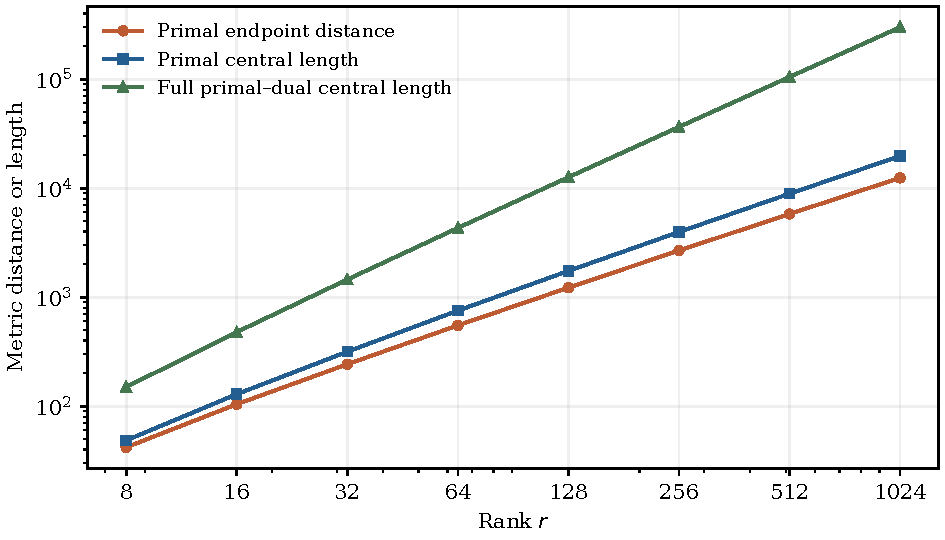
\includegraphics[width=.86\textwidth]{figures/dyadic-lengths.pdf}
 \caption{Numerical values for the dyadic family
 \eqref{eq:dyadic-family}, from $s=0$ to $T=a_r$. The curves show the
 primal endpoint distance $d_U(x^c(0),x^c(T))$ (exact formula), the
 primal central arclength on $[0,T]$ (quadrature), and the full
 central length $\sqrt{2r}\,T$. The first curve is not the distance to
 the whole accurate set, and the third is not the distance to the set
 of feasible small-gap pairs. The orders
 $r\sqrt{\log r}$, $r\log r$, and $r^{3/2}$, and the corresponding step
 counts, follow from \cref{thm:dyadic,thm:completion}.
 Data and generation code accompany the paper.}
 \label{fig:dyadic-lengths}
\end{figure}

\section{What a change of formulation can preserve}
\label{sec:formulation}

\Cref{thm:completion} concerns one formulation and one barrier. This
section gives two movement lower bounds for other formulations,
including those with auxiliary variables. For log-determinant barriers
of symmetric cones, the rank of an exposing dual solution bounds primal
movement; for every logarithmically homogeneous barrier, a bound on the
factor dimensions bounds full primal--dual movement. Neither statement derives a primal
lower bound from an upper bound on the barrier parameter.

\subsection{Exposing dual solutions and free auxiliary variables}
Let $K=\prod_iK_i$ be a product of symmetric cones in Euclidean Jordan
algebras with trace inner products, and let
$\Omega=\{x\in\interior K:Ax=b\}\ne\varnothing$.
Suppose the objective $\ell$ has finite supremum $\ell_*$ over
$\Omega$ and an attained dual solution $s=(s_i)\in K$ that exposes
the optimum:
\begin{equation}
 \ell_*-\ell(x)=\sum_i\ip{s_i}{x_i}\qquad(x\in\Omega).
 \label{eq:exposing-certificate}
\end{equation}
Let $c_i$ be the support idempotent of $s_i$, let
$q_i=\rank(s_i)$, and omit factors of rank zero.
Here $P(c_i)$ is the orthogonal Peirce projection onto the algebra with
unit $c_i$, and $\det_{c_i}$ is its determinant.

\begin{theorem}[Distance bound from the rank of an exposing dual solution]
\label{thm:exposed-rank}
Use the barrier
\[ F(x)=-\sum_i\alpha_i\log\det_i x_i,\qquad \alpha_i\geq1, \]
restricted to $\Omega$. Put $Q_\alpha=\sum_i\alpha_iq_i>0$ and, for
any reference $x^c\in\Omega$, define
\begin{equation}
 \Delta_{c,\alpha}=Q_\alpha
 \left[\prod_i
 \frac{\{\det_{c_i}(s_i)\det_{c_i}(P(c_i)x_i^c)\}^{\alpha_i}}
      {\alpha_i^{\alpha_iq_i}}\right]^{1/Q_\alpha}.
 \label{eq:weighted-exposed-scale}
\end{equation}
For $\eps>0$, every feasible $y$ with objective gap at most $\eps$
satisfies
\begin{equation}
 d_F(x^c,y)\geq\sqrt{Q_\alpha}
            \pos{\log(\Delta_{c,\alpha}/\eps)}.
 \label{eq:exposed-distance}
\end{equation}
The bound does not restrict eigenvalues outside the support of $s$ or
auxiliary variables, and needs no strict complementarity. If a method starts at $x_0$ with
$d_F(x_0,x^c)\leq D_0$ and reaches such a $y$ after $N$ rounds,
each moving the iterate a distance at most $B_0>0$, then
\begin{equation}
 N\geq\frac{\pos{\sqrt{Q_\alpha}\log(\Delta_{c,\alpha}/\eps)-D_0}}{B_0}.
 \label{eq:exposed-rounds}
\end{equation}
In particular, if $\norm{x_0-x^c}_{x^c}\leq\rho$ with $0\leq\rho<1$
and each round has at most $m\in\N$ forward $R$-chords, $0<R<1$,
one can take $D_0=-\log(1-\rho)$ and
$B_0=-m\log(1-R)$.
\end{theorem}
\begin{proof}
We give the compression argument in full to fix the metric
normalization, including the exceptional Jordan algebra. For one idempotent $c$ of
rank $q$, put $a=P(c)x$ and $\phi_c(x)=-\log\det_c a$.
The Hessian of $-\log\det x$ is $P(x^{-1})$ with inverse $P(x)$,
where $P(u)=2L_u^2-L_{u^2}$ is the quadratic representation and
$L_uv=u\circ v$. Since $a^{-1}$ belongs to the Peirce algebra,
\[
 d\phi_c(x)[h]=-\ip{a^{-1}}{h},\qquad
 \norm{d\phi_c(x)}_{x,*}^2=\ip{a^{-1}}{P(x)a^{-1}}=q.
\]
Indeed, the fundamental identity $P(P(u)v)=P(u)P(v)P(u)$ with $u=c$
gives $P(c)P(x)P(c)=P(a)$; then $P(a)a^{-1}=a$ and
$\ip{a^{-1}}{a}=q$. The compression $a$ is positive definite in its
Peirce algebra: if $x\succeq\delta e$, positivity of $P(c)$ gives
$a\succeq\delta c$.
For $\Phi=\sum_i\alpha_i\phi_{c_i}$, the product metric therefore gives
$\norm{d\Phi}_{F,*}^2=Q_\alpha$ before affine restriction and at most
$Q_\alpha$ afterwards. These quadratic-representation identities are
standard~\cite{FarautKoranyi1994}; we do not claim the principal-minor
metric identity as new.

Set $g_i=\ip{s_i}{y_i}>0$ on the active factors. Inside the Peirce
algebra, $z_i=P(s_i^{1/2})P(c_i)y_i$ has trace $g_i$ and determinant
$\det_{c_i}(s_i)\det_{c_i}(P(c_i)y_i)$.
Spectral AM--GM gives
\[
 \det_{c_i}(P(c_i)y_i)
 \leq\det_{c_i}(s_i)^{-1}(g_i/q_i)^{q_i}.
\]
Under $\sum_i g_i\leq\eps$, the weighted product
$\prod_i(g_i/q_i)^{\alpha_iq_i}$ is maximized at
$g_i=\eps\alpha_iq_i/Q_\alpha$. Thus
\[
 \prod_i\det_{c_i}(P(c_i)y_i)^{\alpha_i}
 \leq(\eps/Q_\alpha)^{Q_\alpha}
 \prod_i\alpha_i^{\alpha_iq_i}\det_{c_i}(s_i)^{-\alpha_i}.
\]
Comparing with $x^c$ proves
$\Phi(y)-\Phi(x^c)\geq Q_\alpha\log(\Delta_{c,\alpha}/\eps)$.
Integrating this dual-norm bound along any feasible curve proves \eqref{eq:exposed-distance}. The triangle inequality and \cref{lem:chord-distance} prove the round
statements.
\end{proof}
For unit weights this gives $Q=\sum_iq_i$ and
$\Delta_c=Q[\prod_i\det_{c_i}(s_i)\det_{c_i}(P(c_i)x_i^c)]^{1/Q}$.
The coefficient $\sqrt{Q_\alpha}$ is asymptotically sharp on the full
cone. Apply a quadratic-representation
isometry sending the reference point to the unit element, diagonalize
the transformed dual solution, and multiply its support coordinates by
$t$, keeping the others equal to one. The gap is
$t\ip{s}{e}$ and the curve has length
$\sqrt{Q_\alpha}\log(1/t)$. Together with
\eqref{eq:exposed-distance}, this proves the exact leading coefficient
as $\eps\downarrow0$. An affine slice need not contain this path; we
claim no sharp upper bound on an arbitrary slice.

Hauser and G\"uler's classification
\cite[Theorem~5.5]{HauserGuler2002} states that every self-scaled barrier
on a symmetric cone is, up to an additive constant, a sum of these
log-determinants on its irreducible factors with coefficients
$\alpha_i\geq1$. Thus \cref{thm:exposed-rank} covers every such barrier,
with the weighted scale $\Delta_{c,\alpha}$; replacing $Q$ by $Q_\alpha$
but keeping the unweighted $\Delta_c$ would be incorrect.
The bound depends on the rank of $s$; a general lower bound on the
ranks attainable by different lifted formulations is a separate
question, which the theorem neither assumes nor answers.

\subsection{A bound from factor dimensions for arbitrary cone barriers}
\begin{theorem}[Bounded factor dimension]
\label{thm:dimension-dictionary}
Let a compact full-dimensional convex body $C\subset\R^D$, $D\geq1$,
have an exact affine lift $C=\pi(K\cap\mathcal L)$, where $K$ is a
finite product of proper cones, $\mathcal L$ is an affine subspace,
and $\pi$ is an affine map. Let the minimal face be the smallest face
of $K$ containing $K\cap\mathcal L$; it is a product of faces of the
factors of $K$. Regarding this product as a cone in its linear span and
removing its zero factors gives the reduced product cone. Suppose
each of its factors has dimension at most an integer $d\geq2$.
For $h\geq1$ define
\[
 \Psi_d(h)=2\lfloor h/d\rfloor+\min\{h\bmod d,2\}.
\]
Every logarithmically homogeneous standard self-concordant barrier on
the reduced product cone, including one that couples the factors,
satisfies
\begin{equation}
 \nu\geq\Psi_d(D+1)\geq\frac{2(D+1)}d.
 \label{eq:dimension-parameter}
\end{equation}
For a strictly feasible primal--dual conic pair on this cone, consider
routes from an exact central point with gap $\Delta_0$ to a strictly
feasible pair with gap at most $\eps$, $0<\eps<\Delta_0$. If each
round has at most $m\in\N$ forward $R$-chords in the product metric,
$0<R<1$, the number of rounds is at least
\begin{equation}
 \frac{\sqrt{\Psi_d(D+1)/2}\log(\Delta_0/\eps)}{-m\log(1-R)}.
 \label{eq:dimension-movement}
\end{equation}
\end{theorem}
\begin{proof}
Let $M$ be the dimension of the span of the reduced product cone.
The affine projection of its feasible slice spans $\R^D$, so $M\geq D$.
If $M=D$, the linear part of $\pi$ is invertible on this span, so the
feasible slice has full affine hull and the affine equations impose no
restriction: the feasible slice is the whole reduced cone.
Its invertible affine image is unbounded, contrary to compactness.
Therefore $M\geq D+1$. This elementary argument is consistent
with the classical slack-factorization framework~\cite{GouveiaParriloThomas2013},
but needs no choice of boundary certificates.

Let $r_0$ and $q_0$ be the numbers of ray factors and of factors
of dimension at least two. In each nonray factor choose a two-dimensional linear plane
containing an interior point. Its cone section is proper and
full-dimensional in the plane, hence linearly isomorphic to $\R_+^2$;
its relative interior lies in the factor's interior and its boundary in
the factor's boundary. Together with all rays, these sections give an orthant section of
dimension $r_0+2q_0$ through the interior of the reduced cone.
Restriction preserves standard self-concordance, the degree of
logarithmic homogeneity, and boundary blow-up. The classical orthant parameter lower bound
\cite{NesterovNemirovskii1994,Hildebrand2013} therefore gives
$\nu\geq r_0+2q_0$, even when the original barrier couples factors.
The dimension bound $d$ gives $r_0+dq_0\geq M\geq D+1$.

To solve the integer minimization, write $h=ad+b$, $0\leq b<d$.
For $q_0\leq a$ the smallest possible value of $r_0+2q_0$ is
$2q_0+h-dq_0=h-(d-2)q_0$, minimized at $q_0=a$ and equal to $2a+b$.
For $q_0\geq a+1$ this value is at least $2a+2$, attained with no
rays. The minimum is therefore $2a+\min(b,2)$; the case $b=0$ is
attained with $q_0=a$. Since $\min(b,2)\geq2b/d$, this proves
\eqref{eq:dimension-parameter}. Apply \cref{thm:pd-gap-set} for
\eqref{eq:dimension-movement}.
\end{proof}
The parameter bound concerns barriers on the reduced product cone, not
arbitrary barriers on $C$ or on the affine slice. The theorem combines
classical restriction, dimension, and primal--dual arguments; it does not determine the least dimension of a lift. For a
product of balls, $D=\sum_as_a$, so the bound uses the total ball
dimension and no curvature or regularity assumptions.

\subsection{Grouped balls, norm trees, and PSD packing}
\label{subsec:concrete-formulations}
The following formulations show that fewer conic blocks need not
reduce movement in the given barrier metric. Full proofs,
including all auxiliary variables, are in \cref{app:formulations}.

Take $k$ unit balls, a unit vector $c_a$ for each, and the objective
$\ell=\sum_a\ip{c_a}{w_a}$ with maximum $k$.
For a grouped paraboloid lift, partition each ball's coordinates into
$h$ groups, introduce $q_{aG}=s_{aG}-\norm{w_{aG}}^2>0$ with
$\sum_Gs_{aG}=1$, and use $F=-\sum_{a,G}\log q_{aG}$.
For a PSD packing, place the
$H=kh$ group vectors as columns into real matrix blocks $W_\ell$ in any
arrangement, let every off-diagonal entry of $S_\ell$ be free, and use
\[
 D_\ell=S_\ell-W_\ell^TW_\ell\succ0,\qquad
 F=-\sum_\ell\log\det D_\ell,
 \qquad \sum_{\gamma\text{ from ball }a}(S_{\ell(\gamma)})_{\gamma\gamma}=1.
\]
A group column may be padded with zeros; its free entries are its
group's coordinates. Each group occurs exactly once.
Both barriers are standard self-concordant with exact restricted
parameter $H$; for each, the central path
$z(\tau)=\argmin(F-\tau\ell)$ has
$w_a=r(\tau)c_a$, with
\begin{equation}
 q(\tau)=\frac{2}{\sqrt{h^2+\tau^2}+h},\quad
 r(\tau)=\frac{\tau}{\sqrt{h^2+\tau^2}+h},\quad
 \left\|\frac{dz}{d\log\tau}\right\|^2
   =H\left(1-\frac h{\sqrt{h^2+\tau^2}}\right).
 \label{eq:grouped-packed-center}
\end{equation}
On the path, $q_{aG}=q(\tau)$ (grouped lift) and
$D_\ell=q(\tau)I$ (packing). For every $\tau_0\geq0$ and every
feasible $y$ with gap at most $\eps$,
\begin{equation}
 d_F(z(\tau_0),y)\geq\sqrt H\,
          \pos{\log(q(\tau_0)H/(2\eps))}.
 \label{eq:grouped-packed-distance}
\end{equation}
At the analytic center $\tau_0=0$ the argument of the logarithm is
$k/(2\eps)$, independent of the packing and its off-diagonal
variables.

For a rooted norm tree with $b$ internal nodes, each with at least two
children, use one Lorentz-cone block per internal node:
\begin{equation}
 q_{av}=t_{av}^2-\sum_{u\in I(v)}t_{au}^2
                    -\sum_{j\in J(v)}w_{aj}^2>0,
 \qquad t_{av}>0,
 \qquad t_{a,\mathrm{root}}=1.
 \label{eq:norm-tree-domain}
\end{equation}
Here $I(v)$ and $J(v)$ are the internal and leaf children of $v$.
The positive sheet $t_{av}>0$ is needed for convexity. Use $F=-\sum_{a,v}\log q_{av}$ and
put $L=kb$. Its exact parameter is $\nu=k\nu_T$, where
\begin{equation}
 \nu_T=\begin{cases}2b-2,&\text{the root has only internal children},\\
                         2b-1,&\text{the root has a leaf child}.
          \end{cases}
 \label{eq:tree-parameter}
\end{equation}
Its central path is \eqref{eq:grouped-packed-center} with $h=b,H=L$,
regardless of the tree shape. If $n_v$ counts internal
nodes in the subtree at $v$, including $v$, and $C_{av}=\sum_{j\text{ below }v}c_{aj}^2$, the
internal coordinates are $t_{av}^2=n_vq+r^2C_{av}$.
At the analytic center $\bar z$, $q_{av}=1/b$, and every feasible $y$ with gap at most
$\eps$ satisfies the sharper barrier-value bound
\begin{equation}
 d_F(\bar z,y)\geq\frac{L}{\sqrt\nu}
                        \pos{\log(k/(2\eps))}
 \geq\sqrt{L/2}\,\pos{\log(k/(2\eps))}.
 \label{eq:tree-distance}
\end{equation}
\Cref{app:formulations} proves the exact parameter
\eqref{eq:tree-parameter} by a metric calculation; simply subtracting
the fixed root's contribution from the cone parameter would not be
justified.

For all three formulations, the central path from the analytic center
to objective gap $\eps$ has length
\begin{equation}
 \sqrt{M_0}\,\rho(1-\eps/k)
 =\sqrt{M_0}\log(k/\eps)+O(\sqrt{M_0}),
 \qquad M_0=H\text{ or }L,
 \label{eq:formulation-route}
\end{equation}
for $0<\eps<k$, with the asymptotic form as $\eps/k\downarrow0$.
Sampling this path and the distance bounds give matching forward
$R$-chord counts $\Theta_R(\sqrt{M_0}\log(k/\eps))$, uniformly for $0<\eps\leq k/4$.
An approximate starting point and a fixed number of chords per round
are handled as in \eqref{eq:exposed-rounds}.
These statements concern the given barrier metrics; the block count
alone implies none of these primal lower bounds.

\section{Interpretation}
\label{sec:interpretation}

The comparisons identify three distinct sources of movement. Objective
weights determine which directions become active and at what parameter
scales. Ordered activation can make the central route longer than a
simultaneous motion toward an accurate endpoint. A feasible dual
completion can then require additional movement that is absent from the
primal projection. On the dyadic cube family these effects have separate,
matched asymptotic orders in both length and bounded local moves.

The exact target allocation is useful because a central endpoint need
not be the closest accurate point. It also shows why one aggregate rank
or determinant certificate may be insufficient: the entire objective
weight profile enters the optimum. Conversely, the sharp prefix factor
shows that ordered scalar activation imposes a strong restriction on
how inefficient a central route can be. For equal standard scales the
worst overhead is logarithmic in active rank under a square root, even
when the ambient matrix space is much larger.

Changing a barrier or a formulation requires a new metric comparison.
Optimal parameter alone does not eliminate the centrality cost, as the
canonical cube barriers and the explicit coupled radial family show.
A restriction of a cone barrier can also have much smaller primal
activity than the full homogeneous parameter suggests. The exposed-rank
and concrete-formulation results provide direct lower certificates when
auxiliary motion is permitted, rather than inferring primal cost from an
ambient parameter bound.

All these conclusions retain their stated contracts: fixed barrier
metric, specified starting point, actual terminal accuracy or feasible
duality gap, and bounded starting local norms. Within those contracts,
the explicit shortest routes and matching lower bounds make the cost of
centrality and the cost of dual completion separately measurable.

\appendix
\section{Rational certificates for the scalar dilation}
\label{app:scalar-certificate}
This appendix proves the strict bounds in \eqref{eq:cstar}. All finite
arithmetic checks below are reproduced by the standalone standard-library
script \texttt{scripts/verify\_scalar\_certificate.py}; no floating-point
evaluation is used by the certificate.

\subsection{An elasticity bound}
For $x=\rho^{-1}(y)>0$, define
\[
 E(y)=\frac{yp'(y)}{p(y)},\qquad
 K(y)=\frac{y^2(1-x^2)}{2x^2(1+x^2)}.
\]
Direct differentiation using $p=b'\circ\rho^{-1}$ gives
\begin{equation}
 \frac{\dd E}{\dd\log y}=E-K,\qquad E\geq1,
 \qquad 0<K<1.
 \label{eq:elasticity-ode}
\end{equation}
For the last inequality, set
$B(x)=\sqrt2x\sqrt{(1+x^2)/(1-x^2)}$, so $K=(\rho(x)/B(x))^2$.
With $u=x^2$, the derivative ratio is
\[
 \frac{B'}{\rho'}=\frac{1+2u-u^2}{(1+u)\sqrt{1-u}}>1,
\]
because the difference of squared numerator and denominator is
$u(3+3u-3u^2+u^3)>0$. Equality of the two functions at zero proves
$\rho<B$. Convexity of $p$ gives $E\geq1$, so $E$ increases strictly.
Solving the differential inequality in \eqref{eq:elasticity-ode} on a
multiplicative ray gives $E(ty)>1+t(E(y)-1)$ for $t>1$. Consequently,
for every $a>1$,
\begin{equation}
 \log\frac{p(ay)}{yp'(y)}>
 h_1(E):=\log a+(a-1)(E-1)-\log E.
 \label{eq:elasticity-first}
\end{equation}

For a stronger bound when $E>2$, concavity of the square root gives
\[
 \rho(x)\leq\sqrt2D(x),\qquad
 D(x)=\tfrac32\operatorname{artanh}x-x/2.
\]
At $x=4/5$, $D=(3/2)\log3-2/5<2497/2000$.
Indeed $\log3<1099/1000$ follows by summing the exponential Taylor
polynomial through degree six. Hence
$E(\rho(4/5))<2497\sqrt{41}/8000<2$, the latter inequality being
$2497^2\cdot41<64\cdot2000^2$. Thus $E(y)>2$ implies $x>4/5$.
On this region,
\[
 K\leq G(x):=\frac{D(x)^2(1-x^2)}{x^2(1+x^2)}.
\]
The positive power series for $\operatorname{artanh}$ gives
$D(x)\geq x(1+x^2/2)$, and
$D'(x)=(1+x^2/2)/(1-x^2)$. It follows that
\[
 \tfrac12(\log G)'=
 \frac{D'}D-\frac{x}{1-x^2}-\frac1x-\frac{x}{1+x^2}
 \leq-\frac{x}{1+x^2}<0.
\]
Therefore
\[
 K<G(4/5)<\left(\frac{2497}{2000}\right)^2\frac{225}{656}
 =\frac{56115081}{104960000}<k:=\frac{107}{200}.
\]
This bound holds along the entire multiplicative ray starting at $E>2$.
Integrating \eqref{eq:elasticity-ode} now gives
$E(ty)>k+t(E(y)-k)$ for $t>1$, and hence
\begin{equation}
 \log\frac{p(ay)}{yp'(y)}>h_k(E):=
 k\log a+(a-1)(E-k)-\log E\qquad(E>2).
 \label{eq:elasticity-second}
\end{equation}

\subsection{The strict upper certificate}
Take $a=69/50$. On $1\leq E\leq2$, $h_1$ is decreasing, and
\[
 h_1(E)\geq h_1(2)=\log(69/100)+19/50>0,
\]
because
$e^{19/50}>1+19/50+(19/50)^2/2=7261/5000>100/69$.
On $E>2$, the convex function $h_k$ has its global minimum at $E=50/19$,
where its value is
\[
 \log(19/50)+1+\frac{107}{200}\bigl(\log(69/50)-19/50\bigr).
\]
The positive series
$\log((1+z)/(1-z))=2\sum_{j\geq0}z^{2j+1}/(2j+1)$ yields, with
$r_0=31/69$ and $s_0=19/119$,
\begin{align*}
 \log(19/50)&>
 -2\left(r_0+\frac{r_0^3}3+\frac{r_0^5}{5(1-r_0^2)}\right)
 =-\frac{9064603453}{9362506500},\\
 \log(69/50)&>2(s_0+s_0^3/3)=\frac{1628072}{5055477}.
\end{align*}
Substitution leaves the strictly positive rational lower bound
\begin{equation}
 h_k(50/19)>
 \frac{255839420916449}{315546241820670000}>0.
 \label{eq:upper-certificate-margin}
\end{equation}
Thus $p((69/50)y)>yp'(y)$ for every $y>0$. Since the maximum defining
$c_\star$ is attained, the upper bound on $c_\star$ is strict.

\subsection{The strict lower certificate}
The elementary transform in \eqref{eq:scalar-elementary} has series
\begin{equation}
 Y(z)=\sum_{j\geq0}\frac{(2-2^{-j})z^{2j+1}}{2j+1},\qquad
 S_N(z)<Y(z)<S_N(z)+\frac{2z^{2N+3}}{(2N+3)(1-z^2)}.
 \label{eq:Y-rational-series}
\end{equation}
Here $S_N$ includes $j=0,\ldots,N$; the tail estimate follows by bounding
$2-2^{-j}<2$ and every tail denominator by $2N+3$.
Set
\[
 v_0=\frac{3787}{4000},\quad w_0=\frac{9797031}{10^7},\quad
 a_0=\frac{68743}{50000}.
\]
Summation through $N=1200$ and rational squaring for $A$ verify
\begin{gather*}
 \frac{2453756741730599}{10^{15}}<Y(v_0)
 <\frac{12268783708653}{5\cdot10^{12}},\qquad
 \frac{134943211257327}{4\cdot10^{13}}<Y(w_0),\\
 A(v_0)>\frac{405367307458211}{4\cdot10^{13}},\qquad
 A(w_0)<\frac{25381942601625079}{10^{15}}.
\end{gather*}
These finite enclosures imply
\begin{align}
 Y(w_0)-a_0Y(v_0)&>
 \frac{2071874360571}{250000000000000000}>0,\notag\\
 Y(v_0)A(v_0)-w_0A(w_0)&>
 \frac{2049519399569150216498389}{40000000000000000000000000000}>0.
 \label{eq:lower-certificate-margins}
\end{align}
The second inequality states $P(w_0)<Y(v_0)A(v_0)$.
Since $P$ and $Y$ are strictly increasing, it follows that
$Y(W(v_0))>Y(w_0)>a_0Y(v_0)$. This is a strictly feasible witness for
$c_\star>a_0$. The interval bounds, tail estimate, and rational squaring
are a finite proof certificate, independent of a numerical optimizer or
an assumption about stationary-point uniqueness.

\subsection{Every scalar-dilation maximizer lies in a certified interval}
The same inequalities also locate every maximizer of the distinct
standard-barrier constant $c_\star$. Keep $a_0=68743/50000$
and $k=107/200$ in \cref{eq:elasticity-first,eq:elasticity-second}.
Exact positive-series bounds for logarithms give
\begin{align*}
 h_1(2)&>2589087717927/40000000000000000>0,\\
 h_k(571/250)&>2011885403423/100000000000000000>0,\\
 h_k(773/250)&>8579961311243/500000000000000000>0.
\end{align*}
For clarity these are finite certificates: for rational $q\in(0,1)$,
the partial sum of $2\sum_{j\geq0}q^{2j+1}/(2j+1)$ through
$j=N$ bounds $\log((1+q)/(1-q))$ below, and adding
$2q^{2N+3}/[(2N+3)(1-q^2)]$ bounds it above. Taking
$q=(z-1)/(z+1)$ for $z=a_0,2,571/250,773/250$ and $N=200$
verifies the displayed inequalities using rational arithmetic.
The function $h_1$ decreases on $[1,2]$. The convex function
$h_k$ decreases until $E=1/(a_0-1)$ and increases thereafter;
this minimum lies strictly between $571/250$ and $773/250$.
Therefore a scalar ratio greater than $a_0$ is possible only for
$571/250<E<773/250$.

In the coordinate of \eqref{eq:scalar-elementary}, $E=Y(v)/v$
is strictly increasing by \eqref{eq:elasticity-ode}.
The series \eqref{eq:Y-rational-series} through $N=1200$ gives
\begin{align*}
 \frac{571}{250}\frac{4611}{5000}-Y(4611/5000)
 &>159652343530451/200000000000000000>0,\\
 Y(9701/10000)-\frac{773}{250}\frac{9701}{10000}
 &>19492543073837/250000000000000000>0.
\end{align*}
Since every global maximizer has ratio $c_\star>a_0$, these
inequalities, followed by rational squaring in
$x=v/\sqrt{2-v^2}$, prove
\begin{equation}
 \frac{4611}{5000}<v_\star<\frac{9701}{10000},\qquad
 \frac{43}{50}<x_\star<\frac{943}{1000}.
 \label{eq:cstar-maximizer-location}
\end{equation}
The verification script includes every displayed bound. Finally,
differentiating $P(W(v))=Y(v)A(v)$ shows that every stationary
point satisfies
\[
 Y(v)[Y'(v)A(v)+Y(v)A'(v)]
 =Y(W(v))Y'(v)A(W(v)),\qquad
 A'(v)=\frac{v(3-v^2)}{(1-v^2)^2\sqrt{2-v^2}}.
\]
No uniqueness of this stationary point or of the $c_\star$
maximizer is inferred from its certified localization.

\section{The scalar envelope and a barrier with nonmonotone speed}
\label{app:barrier-profiles}
\begin{proposition}[Exact envelope for a relaxed problem with constant $k=\log2$]
\label{prop:scalar-envelope}
Let $p\in C^2([0,\infty))$ satisfy $p(0)=0$, $p'>0$, $|p''|\leq p'$, and $p\leq p'$ on
$[0,\infty)$. Put $k=\log2$ and
\begin{equation}
 C(a)=\begin{cases}
 1+\displaystyle\frac1a\log\frac{k}{k(2-e^{-a})-a},
       &2a\leq k(2-e^{-a}),\\[5pt]
 1+\displaystyle\frac1a\log\frac{4a}{k(2-e^{-a})^2},
       &2a\geq k(2-e^{-a}).
 \end{cases}
 \label{eq:scalar-envelope-C}
\end{equation}
Then $C_{\SC}=\max_{a>0}C(a)$ has a unique maximizer, is strictly below two,
and
\[
 a\leq p^{-1}(ap'(a)/k)\leq C(a)a\leq C_{\SC}a.
\]
For the $C^2$ function $p$, put $\upsilon=p/p'$. The function $C(a)$ is
the exact envelope when $\upsilon$ is relaxed to any locally absolutely
continuous function $\upsilon:[0,\infty)\to[0,1]$ satisfying
\begin{equation}
 \upsilon(0)=0,\quad0<\upsilon(y)\leq1\quad(y>0),\qquad
 1-\upsilon\leq\upsilon'\leq1+\upsilon\quad\text{a.e.}
 \label{eq:upsilon-envelope}
\end{equation}
This exactness holds for the fixed constant $k$; it is not a claim about
the optimal arclength constant for products of copies of one smooth
barrier.
\end{proposition}
\begin{proof}
The derivative identity $\upsilon'=1-\upsilon p''/p'$ gives
\eqref{eq:upsilon-envelope}. Integration yields
\[
 1-e^{-a}\leq\upsilon(a)\leq\min(1,e^a-1),\qquad
 \frac{\upsilon(a)}a\leq\frac1k.
\]
For the last inequality, $(e^a-1)/a$ increases and $1/a$ decreases;
their crossing is at $a=k$. Thus the comparison point $a+t$,
defined by $p(a+t)=ap'(a)/k$, has $t\geq0$. Write
$u=\upsilon(a)$ and integrate $(\log p)'=1/\upsilon$:
\begin{equation}
 \int_0^t\frac{\dd q}{\upsilon(a+q)}=\log\frac{a}{ku}.
 \label{eq:envelope-time}
\end{equation}
The upper bound $\upsilon'\leq1+\upsilon$ and the cap $\upsilon\leq1$
give
$\upsilon(a+q)\leq m_u(q):=\min\{1,(1+u)e^q-1\}$.
The cap is reached at $q_u=\log(2/(1+u))$. For $t\leq q_u$,
\[
 \int_0^t\frac{\dd q}{m_u(q)}
 =\log\frac{(1+u)-e^{-t}}u.
\]
For $t\geq q_u$, the integral equals $\log((1+u)/(2u))+t-q_u$.
The right side of \eqref{eq:envelope-time} is fixed, and the actual
integral is at least this envelope integral. Solving the latter
therefore gives an upper bound on $t$:
\[
 t\leq\begin{cases}
 \log\dfrac{k}{k(1+u)-a},&2a\leq k(1+u),\\[3pt]
 \log\dfrac{4a}{k(1+u)^2},&2a\geq k(1+u).
 \end{cases}
\]
Both expressions decrease with $u$, and their values and first
derivatives agree at the switch. Substitute $u\geq1-e^{-a}$ to
obtain \eqref{eq:scalar-envelope-C}.

The two branches meet at exactly one positive point: $2a-k(2-e^{-a})$
has positive derivative $2-ke^{-a}$ and changes sign. It lies below $k$.
On the first branch, $C(a)<2$ is equivalent to
$2k(1-e^{-a})-a>0$. This strictly concave function vanishes at
$0$ and $k$, and the branch has $0<a<k$. On the second branch,
$C(a)<2$ is equivalent to
\[
 k(4e^a-4+e^{-a})-4a>0.
\]
Since $k>2/3$, the expression exceeds
$(2/3)(4e^a+e^{-a}-4-6a)$. The inequalities
$e^a\geq1+a+a^2/2+a^3/6$ and $e^{-a}\geq1-a$ bound the
parenthesis below by $1-3a+2a^2+(2/3)a^3$. Its minimum on
$[0,\infty)$ is $(16-5\sqrt{10})/3>0$, as differentiation shows.
Here $k>2/3$ follows, for example, from the first term of the
positive series for $\log2=2\operatorname{artanh}(1/3)$.

The two branches are continuously differentiable at their common
boundary. Their endpoint limits are $1/k$ as $a\downarrow0$ and
$1$ as $a\to\infty$. Moreover
$C(k)=1+k^{-1}\log(16/9)>1/k$, because
$\log(32/9)>1$ (use $e<3<32/9$).
Hence continuity proves a maximum at a finite positive argument,
and the strict pointwise bound implies $C_{\SC}<2$.
To prove uniqueness and to evaluate $C_{\SC}$ numerically, write $C=1+B/a$, where $B$ is
the logarithm on the appropriate branch. An interior stationary
point satisfies $aB'=B$, with
\[
 B'=\frac{1-ke^{-a}}{k(2-e^{-a})-a}\quad\hbox{or}\quad
 B'=\frac1a-\frac{2e^{-a}}{2-e^{-a}}.
\]
On the first branch, $B=-\log(2-e^{-a}-a/k)$ is strictly
convex, since its positive logarithm argument has second derivative
$-e^{-a}<0$. As $B(0)=0$, $aB'-B>0$ there. On the second,
\[
 B''=-\frac1{a^2}+\frac{4e^{-a}}{(2-e^{-a})^2}<0.
\]
Indeed the strict inequality is equivalent to
$2e^{a/2}-e^{-a/2}>2a$; the Taylor bounds
$e^t\geq1+t+t^2/2$ and $e^{-t}\leq1-t+t^2/2$ for $t\geq0$
give a difference at least $1-a/2+a^2/8>0$.
Thus $aB'-B$ strictly decreases on the second branch, starts
positive by continuous differentiability at the switch, and tends
to $-\infty$. It has one zero, which is the unique global maximizer.
Numerical evaluation gives $a\approx0.65011438345$ and
$C_{\SC}\approx1.831856423$; these decimals are not used in the
bound or in its attainment proof.

Finally, for fixed $a$ take $\upsilon(y)=1-e^{-y}$ until $a$,
then follow $\upsilon'=1+\upsilon$ until reaching one, and
remain one thereafter. This continuous, piecewise differentiable
function obeys \eqref{eq:upsilon-envelope} almost everywhere and
attains every envelope equality used at $a$. Reconstruct $p$ by
$(\log p)'=1/\upsilon$, with normalization $p'(0)=1$;
the behavior $\upsilon(y)=y+O(y^2)$ gives a well-defined positive
solution with $p(0)=0$. This proves exactness for the stated relaxed
problem. Likewise, $k$ is the largest constant valid for all
admissible functions $\upsilon$, since the admissible function
$\upsilon=\min(1,e^y-1)$ attains $\inf_y y/\upsilon(y)=k$. These two
extremal functions need not come from one fixed smooth scalar barrier.
\end{proof}

\subsection{A smooth barrier whose central speed is not monotone}
\label{app:nonmonotone-construction}
For $A>4$ define, for all real $y$,
\[
 P_A(y)=\frac{1+2e^{-A}\cosh y}{1+2e^{-A}},\quad
 X_A(y)=\int_0^y\frac{\dd u}{P_A(u)},\quad
 Z_A(y)=\int_0^y P_A(u)\dd u.
\]
The map $X_A$ is a smooth increasing bijection from $\R$ onto
a finite interval $(-b_A,b_A)$: $P_A(y)\geq
e^{y-A}/(1+2e^{-A})$ for $y\geq0$, and $P_A$ is even.
Define $f_A$ by $f_A'(X_A(y))=Z_A(y)$ and $f_A(0)=0$.
All these functions are smooth, so no piecewise smoothing or boundary
extension is needed.
Differentiation gives
\begin{equation}
 f_A''(X_A(y))=P_A(y)^2,
 \quad\frac{|f_A'''|}{(f_A'')^{3/2}}=
        2\frac{|P_A'|}{P_A}<2,
 \quad V_A(y):=\frac{f_A'}{\sqrt{f_A''}}
 =\frac{y+2e^{-A}\sinh y}{1+2e^{-A}\cosh y}.
 \label{eq:nonmonotone-barrier}
\end{equation}
In particular, $y$ is the exact metric coordinate of $f_A$, and $0$ is
its analytic center. Since $V_A(y)\to\pm1$ as $y\to\pm\infty$,
the identity $\frac{\dd}{\dd y}f_A(X_A(y))=V_A(y)$ proves blow-up
at both endpoints. Also $Z_A(y)\to\pm\infty$,
so $f_A'$ takes every real value.

The exact parameter of $f_A$ is $\nu_A=\sup_y V_A(y)^2$.
For $0\leq y\leq A$, $V_A(y)\leq y+1\leq A+1$.
For $y=A+u\geq A$, use $2e^{-A}\sinh y\leq2e^{-A}\cosh y$
and $2e^{-A}\cosh y\geq e^u$ to get
\[
 V_A(y)\leq1+\frac{A+u-1}{1+e^u}\leq A+1;
\]
the final inequality follows from $u-1\leq Ae^u$ for $A>4$.
Oddness handles negative $y$. At $y=A/2$, the denominator in
\eqref{eq:nonmonotone-barrier} is
$1+e^{-A/2}+e^{-3A/2}<3/2$, so $V_A(A/2)>A/3$.
Thus $A^2/9<\nu_A\leq(A+1)^2$. The speed $V_A$ is not monotone:
it exceeds one at $A/2$ but tends to one at the endpoint.

Fix $r$ and $0<\delta<1/2$. Uniformly for
$y\in[\delta A,(1-\delta)A]$ as $A\to\infty$,
$P_A(y)=1+o(1)$ and $Z_A(y)=y+o(1)$.
Consequently, while the metric coordinate crosses this interval, the
logarithmic central-path parameter increases by
\[
 \log Z_A((1-\delta)A)-\log Z_A(\delta A)
 =\log\frac{1-\delta}{\delta}+o(1).
\]
Choose $B>\log((1-\delta)/\delta)$ and weights with
$\log w_i=B(r-i)$, and stop the central path at
$s_1=\log Z_A((1-\delta)A)$. For large $A$, the $r$ parameter windows,
shifted by the weights, are disjoint, and in each one metric coordinate
advances by $(1-2\delta)A$. Therefore the central arc has length at
least $r(1-2\delta)A$.

At the final parameter, $Z_A(y_i)=Z_A((1-\delta)A)e^{B(r-i)}$.
For $y\geq\delta A$ and large $A$,
$Z_A(y)\geq e^{y-A}/3$ and
$Z_A((1-\delta)A)<A$. Thus
$y_i\leq A+\log(3A)+B(r-i)$, so the endpoint distance is at most
$\sqrt r[A+\log(3A)+Br]$.
Let $A\to\infty$ with $r,\delta,B$ fixed, then let
$\delta\downarrow0$. The ratio approaches $\sqrt r$, proving
\cref{prop:nonmonotone}. This does not contradict comparisons that
depend on the barrier parameter, such as \eqref{eq:NN-comparison}: the
scalar parameter, and hence the product parameter $r\nu_A$, diverges in
this construction.

\section{Proofs for the concrete formulations}
\label{app:formulations}

\subsection{Grouped paraboloids and arbitrary PSD column packing}
For a grouped tangent $(\dot s,\dot w)$, put
$\dot q=\dot s-2\ip{w}{\dot w}$. Direct differentiation gives
\begin{equation}
 D^2(-\log q)[(\dot s,\dot w),(\dot s,\dot w)]
       =(\dot q/q)^2+2\norm{\dot w}^2/q.
 \label{eq:grouped-metric}
\end{equation}
For a packed block, an arbitrary affine tangent gives
$\dot D=\dot S-\dot W^TW-W^T\dot W$, and
\begin{equation}
 D^2(-\log\det D)[(\dot S,\dot W),(\dot S,\dot W)]
 =\tr((D^{-1}\dot D)^2)
       +2\tr(D^{-1}\dot W^T\dot W).
 \label{eq:packing-metric}
\end{equation}
These are Hessians in affine $(s,w)$ or $(S,W)$ coordinates; treating
$D$ as an independent affine variable when taking the second derivative
would omit the second term. With $c_\ell$ columns in block $\ell$,
trace Cauchy--Schwarz gives
\begin{equation}
 \norm{\dot z}_F^2\geq
 \sum_\ell\frac1{c_\ell}
            \left(\frac{\mathrm d}{\mathrm dt}\log\det D_\ell\right)^2.
 \label{eq:packing-contraction}
\end{equation}
Its scalar version is the simultaneous contraction onto every $\log q$.
Both Hessians are positive definite on the free affine coordinates.
Standard self-concordance follows by restricting the classical PSD
barrier to the affine matrices
$\left(\begin{smallmatrix}I&W\\W^T&S\end{smallmatrix}\right)$, whose
determinant is $\det D$; the one-column case gives \eqref{eq:grouped-metric}.
The derivative $DF=-\sum_\ell\tr(D_\ell^{-1}\dot D_\ell)$ and
\eqref{eq:packing-contraction} imply
$|DF[\dot z]|\leq\sqrt H\norm{\dot z}_F$, where
$H=\sum_\ell c_\ell=kh$. This proves the parameter upper bound $H$
without charging the fixed identity blocks.

For a feasible target write $\delta_a=1-\ip{c_a}{w_a}$.
The diagonal residuals $d_\gamma=(D_{\ell(\gamma)})_{\gamma\gamma}$
satisfy
\[
 \sum_{\gamma\text{ from }a}d_\gamma=1-\norm{w_a}^2
 \leq1-\ip{c_a}{w_a}^2\leq2\delta_a.
\]
The same identity holds for grouped $q_{aG}$. If the target error is
at most $\eps$, then $\sum_a\delta_a\leq\eps$ and
\begin{equation}
 \prod_\ell\det D_\ell
 \leq\prod_\gamma d_\gamma
 \leq\prod_a(2\delta_a/h)^h
 \leq(2\eps/H)^H.
 \label{eq:packing-collapse}
\end{equation}
The first inequality is Hadamard's inequality and permits every
completion variable to vary; it is not a diagonal-fiber assumption.
Integrating \eqref{eq:packing-contraction} and using weighted
Cauchy--Schwarz shows that every joining curve has length at least
$H^{-1/2}$ times the absolute change in the sum of log determinants.
If the reference has $D_\ell=q_0I$,
\eqref{eq:packing-collapse} gives \eqref{eq:grouped-packed-distance}.

For completeness, these are indeed the claimed centers. At fixed $W$
and fixed residual diagonals, Hadamard's inequality minimizes the
barrier precisely when every residual $D_\ell$ is diagonal.
Partial minimization over the unrestricted off-diagonal entries of $S$
therefore leaves the grouped problem. Its equations in $s_{aG}$ give
one common residual $q$ per ball, and its equations in $w$ give
$w_{aG}=(\tau q/2)c_{aG}$. The source equation becomes
$hq+(\tau q/2)^2=1$, proving \eqref{eq:grouped-packed-center}.
Positive definite Hessians make these stationary points the unique
centers. Differentiated central stationarity on the affine slice yields
$H_\tau z'(\tau)=\nabla\ell$ and hence
\[
 \left\|\frac{dz}{d\log\tau}\right\|^2
 =\tau^2\frac{\mathrm d}{\mathrm d\tau}\ell(z(\tau))
 =k\tau^2r'(\tau)
 =H\left(1-\frac h{\sqrt{h^2+\tau^2}}\right).
\]
At a center, $DF=\tau\,d\ell$ on the slice, so the same expression is
the squared dual gradient norm. Its limit $H$ proves the exact parameter.
Changing variables from $\tau$ to $r$ gives the length element
$\sqrt H\rho'(r)\dd r$, proving \eqref{eq:formulation-route}.

\subsection{Linked norm-tree centers and distance}
The positive-sheet domain \eqref{eq:norm-tree-domain} is a convex affine
restriction of a product of Lorentz cones. Its Hessian is positive
definite: any nonzero free direction changes at least one cone block,
whose Hessian is positive definite. Restriction and addition preserve
standard self-concordance. Telescoping cancels every nonroot internal
square and gives, for each source,
\begin{equation}
 \sum_vq_{av}=1-\norm{w_a}^2.
 \label{eq:tree-telescoping}
\end{equation}
The derivative in a nonroot axial variable is
$-2t_{av}/q_{av}+2t_{av}/q_{a,\mathrm{parent}(v)}$.
Since $t_{av}>0$, central stationarity forces all residuals in a tree
to agree. Leaf stationarity gives $w_a=rc_a$, and
\eqref{eq:tree-telescoping} becomes $bq+r^2=1$, with $r=\tau q/2$.
The positive internal coordinates are uniquely
$t_{av}=(n_vq+r^2C_{av})^{1/2}$; their root value is one.
These equations prove feasibility and stationarity, and strict convexity
proves uniqueness. They give the analytic center $w=0,t_{av}^2=n_v/b$
and the path/speed formulas asserted in the main text.

For each Lorentz block, the parameter-two gradient inequality gives
$(d\log q_{av})^2\leq2D^2(-\log q_{av})$ after restriction.
Therefore the total metric controls the Euclidean log-residual metric
with factor $1/\sqrt2$. More sharply, with the exact restricted
parameter $\nu$ proved below, the barrier itself is
$\sqrt\nu$-Lipschitz in metric length. Telescoping and the same source
AM--GM calculation as \eqref{eq:packing-collapse} give
\[
 \prod_{a,v}q_{av}(y)\leq(2\eps/L)^L,\qquad
 F(y)-F(\bar z)\geq L\log(k/(2\eps)).
\]
This proves \eqref{eq:tree-distance}. Differentiated stationarity gives
the same speed as for grouped balls with $h=b,H=L$, so the same scalar
integration proves \eqref{eq:formulation-route}. Thus no asymptotic
regularity of boundary KKT equations is needed for the matched route.

\subsection{Exact root-slice parameter}
We prove \eqref{eq:tree-parameter} for one tree. Before fixing the root
$t$, let $\Phi=-\sum_v\log q_v$ on the linked cone and $H=\Phi''$.
Its logarithmic degree is $2b$; hence
$H z=-\Phi'(z)$ and $\norm{\Phi'}_{H^{-1}}^2=2b$.
Let $e_t$ be the root-coordinate covector. Orthogonal projection of the
gradient onto $\{h:e_t^Th=0\}$ gives the exact restricted norm
\begin{equation}
 \norm{DF}_{F,*}^2=2b-\frac{t^2}{e_t^TH^{-1}e_t},\qquad
 \nu_T=2b-\frac1{\sup_z\beta_T(z)},\qquad
 \beta_T(z)=\frac{e_t^TH^{-1}e_t}{t^2}.
 \label{eq:root-leverage}
\end{equation}
Dikin containment and the halfspace $t>0$ imply
$e_t^TH^{-1}e_t\leq t^2$, so $\beta_T\leq1$.
Indeed, if the inequality failed, a vector of local norm less than one
could move the root coordinate to zero.

If a root child is a free leaf, set $t=1$ and that leaf to
$\sqrt{1-\delta}$. Set other root leaves to zero and scale every
internal child subtree from a fixed interior point by $\delta^2$.
The root residual is $q=\delta-O(\delta^4)>0$.
For the ambient trial direction $h_t=1$, $h_{\rm leaf}=1$, and every
other component zero, descendant blocks contribute zero, while
\[
 D^2\Phi[h,h]
 =\frac{\{2(1-\sqrt{1-\delta})\}^2}{q^2}\longrightarrow1.
\]
Here the root residual's second derivative in that direction is zero.
The variational identity
$(e_t^TH^{-1}e_t)^{-1}=\min_{h_t=1}h^THh$ now gives
$\sup\beta_T=1$. This includes a one-node tree without descendants.
It proves $\nu_T=2b-1$ with an explicit feasible limiting sequence.

Suppose instead that all root children are internal, with positive
axial coordinates $a_1,\ldots,a_c$. Eliminate all their strict
descendants from the Hessian. The effective axial curvature $h_i$ of
child subtree $i$ is at least $a_i^{-2}$ by the same Dikin halfspace
argument on that subtree. Increasing an axial curvature increases the
root Schur complement, so a lower bound is obtained from
\[
 -\log(t^2-\textstyle\sum_i a_i^2)-\sum_i\log a_i.
\]
Normalize $t=1$, put $r=\sum_i a_i^2$, $q=1-r$, and
$Z=\sum_i a_i^4/(q+2a_i^2)$. Its child Hessian is a diagonal matrix
with entries $2/q+a_i^{-2}$ plus $4aa^T/q^2$; the root cross row is
$-4a^T/q^2$, and the root entry is $2(1+r)/q^2$.
The rank-one inverse formula therefore gives the root Schur complement
\begin{equation}
 S=\frac{2(1+r)-16Z/(q+4Z)}{q^2}.
 \label{eq:root-schur}
\end{equation}
Since $x/(q+2x)$ increases in $x\geq0$,
$\sum_i a_i^4/(q+2a_i^2)\leq r^2/(q+2r)=r^2/(1+r)$.
The inequality $S\geq2$ is equivalent to
$r(3-r)\geq4(2-r)Z$; replacing $Z$ by this upper bound leaves
$3r(1-r)^2/(1+r)\geq0$. Thus $\beta_T\leq1/2$.
Conversely, scale all child subtrees by $\delta\downarrow0$.
The trial direction $h_t=1$, with all other variables fixed, has norm
squared $2(1+r)/(1-r)^2\to2$.
Together with the lower bound on the minimizing Schur complement this
proves $\sup\beta_T=1/2$ and $\nu_T=2b-2$.
For independent trees, gradient norm squares and their suprema add,
proving the product parameter used in \eqref{eq:tree-distance}.

\subsection{Heterogeneous source counts and objective weights}
A single weighted version records the dependence on source sizes for
all three formulations. Let source $a$ have $m_a$ groups or internal
nodes, let $M_0=\sum_am_a$, $p_a=m_a/M_0$, and maximize
$\sum_a\lambda_a\ip{c_a}{w_a}$ with every $\lambda_a>0$.
Define the scale
\begin{equation}
 \Delta_{\rm eff}=\prod_a(\lambda_a/p_a)^{p_a}.
 \label{eq:formulation-entropy}
\end{equation}
At the separate analytic centers all source residuals are $1/m_a$.
For an accurate target, put
$e_a=\lambda_a(1-\ip{c_a}{w_a})$, so $\sum_a e_a\leq\eps$.
Telescoping, or the residual diagonal identities and Hadamard's
inequality, show that the ratio of terminal to central residual products
is at most
$\prod_a(2e_a/\lambda_a)^{m_a}$.
This product is maximized at $e_a=\eps p_a$, giving
\[
 F(y)-F(\bar z)\geq M_0\log(\Delta_{\rm eff}/(2\eps)).
\]
Consequently the entire accurate set is at distance at least
\begin{equation}
 \frac{M_0}{\sqrt\nu}\pos{\log(\Delta_{\rm eff}/(2\eps))},
 \quad
 \nu=\begin{cases}M_0,&\text{grouped or packed},\\
                   \sum_a\nu_{T_a},&\text{norm trees}.
       \end{cases}
 \label{eq:heterogeneous-formulation-distance}
\end{equation}
The grouped/packed parameter remains exact by applying the center
calculation source by source, with parameter $\tau\lambda_a$.
For equal weights $\lambda_a=\lambda>0$,
$\Delta_{\rm eff}=\lambda\exp(-\sum_ap_a\log p_a)$;
weighted AM--GM gives $\Delta_{\rm eff}\leq\sum_a\lambda_a$ with
equality precisely when $\lambda_a$ is proportional to $m_a$.
Thus the scale, as well as the square-root count, matters for movement.

\bibliographystyle{plainnat}
\bibliography{bibliography}
\end{document}
